
\newcommand{\bSigma}{\bm{\Sigma}}
\newcommand{\bmu}{\bm{\mu}}
\renewcommand{\bx}{\bm{x}}
\newcommand{\by}{\bm{y}}
\newcommand{\bX}{\bm{X}}
\newcommand{\bI}{\bm{I}}
\newcommand{\bw}{\bm{w}}
\newcommand{\ba}{\bm{a}}
\newcommand{\bb}{\bm{b}}
\newcommand{\bk}{\bm{k}}  
\newcommand{\inv}{^{-1}}

\renewcommand{\norm}{{\mathcal{N}}}

\renewcommand\transpose{^{\textrm{\tiny{\sf{T}}}}}
\newcounter{defcounter} % To define equation number according to rasmussen

%\usefonttheme[onlymath]{serif}

\begin{frame}[c]{}

\centering
\huge
Lecture 6:\\
Bayesian linear regression and Gaussian processes
\end{frame}
%----------------------------------------------------------------------
\begin{frame}[c]{Where are we? The big picture}

\begin{itemize}
	\item Introduction
	\item Background
	\begin{itemize}
		\item Design spaces in ML
		\item Evaluation and visualization
	\end{itemize}
	\item[$\to$] Hyperparameter optimization (HPO)
	\begin{itemize}
		\item[$\to$] Bayesian optimization
		\item Other black-box techniques
		%\item \strikethrough{Speeding up HPO with multi-fidelity optimization}
		\item More details on Gaussian processes
	\end{itemize}
	\item Pentecost (Holiday) -- no lecture
	\item Architecture search I + II
	\item Meta-Learning
	\item Learning to learn $\&$ optimize
	\item Beyond AutoML: algorithm configuration and control
	\item Project announcement and closing
\end{itemize}

\end{frame}
%----------------------------------------------------------------------

%%%%%%%%%%%%%%%%%%%%%%%%%%%%%%%%%%%%%%%%%%%%%%%%%%%%%%%%%%%%%%%%%%%%%%%%%

\section*{Introduction}
\begin{frame}
\frametitle{Today's Learning Goals}
After today's lecture, you can ...
\begin{itemize}
\item Derive Bayesian linear regression
\item Derive Gaussian processes
\item Explain the relationship between Bayesian linear regression and Gaussian processes
\end{itemize}

\end{frame}

%%%%%%%%%%%%%%%%%%%%%%%%%%%%%%%%%%%%%%%%%%%%%%%%%%%%%%%%%%%%%%%%%%%%%%%%%

\begin{frame}
\frametitle{Resources}
Today's material is based on:
\begin{itemize}
\item Chapter 2 of \\ \textit{Gaussian Processes for Machine Learning}, Carl Edward Rasmussen and Christopher K. I. Williams\footnote{\url{http://www.gaussianprocess.org/gpml/}}
\item Another excellent resource: Philipp Hennig’s Gaussian process tutorials\footnote{\url{http://ei.is.tuebingen.mpg.de/person/phennig}}

\end{itemize}
\end{frame}

%%%%%%%%%%%%%%%%%%%%%%%%%%%%%%%%%%%%%%%%%%%%%%%%%%%%%%%%%%%%%%%%%%%%%%%%%

\section{The Gaussian distribution}
\begin{frame}

\begin{block}{The univariate form}
\[f(x) = \frac{1}{\sigma\sqrt{2\pi}} \exp \left(-(\frac{x-\mu)^2}{2\sigma^2}\right)\]
\end{block}
\begin{center}
Named after Carl Friedrich Gauss (1777-1855)
\begin{figure}
    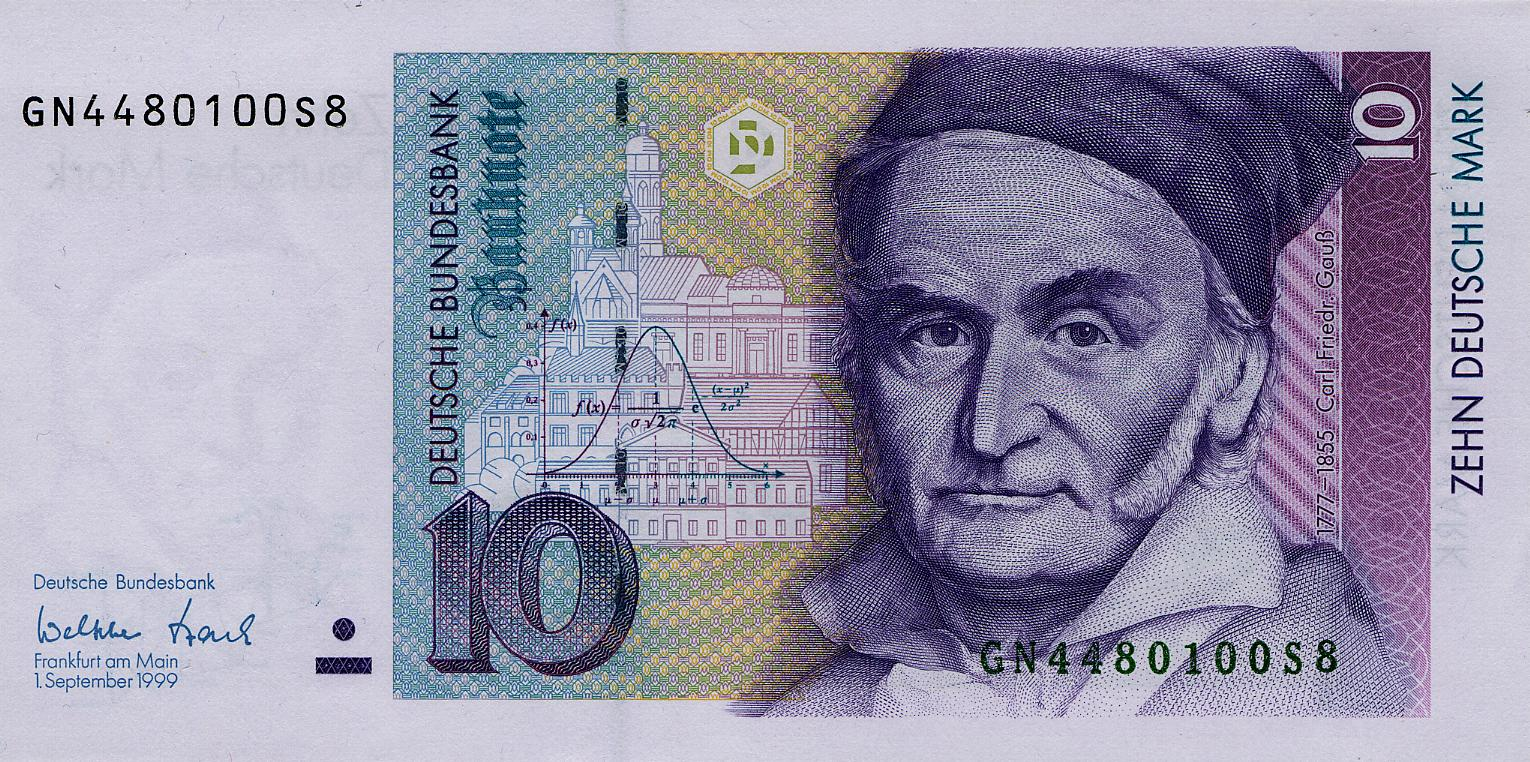
\includegraphics[width=0.5\textwidth]{images/plots/10-Deutsche-Mark.jpg}
    \caption{Wikipedia, public domain}
\end{figure}
\end{center}

\end{frame}

%%%%%%%%%%%%%%%%%%%%%%%%%%%%%%%%%%%%%%%%%%%%%%%%%%%%%%%%%%%%%%%%%%%%%%%%%
\begin{frame}
\begin{block}{The univariate form}
\[f(x) = \frac{1}{\sigma\sqrt{2\pi}} \exp \left(-\frac{(x-\mu)^2}{2\sigma^2}\right)\]
\end{block}

\begin{figure}
    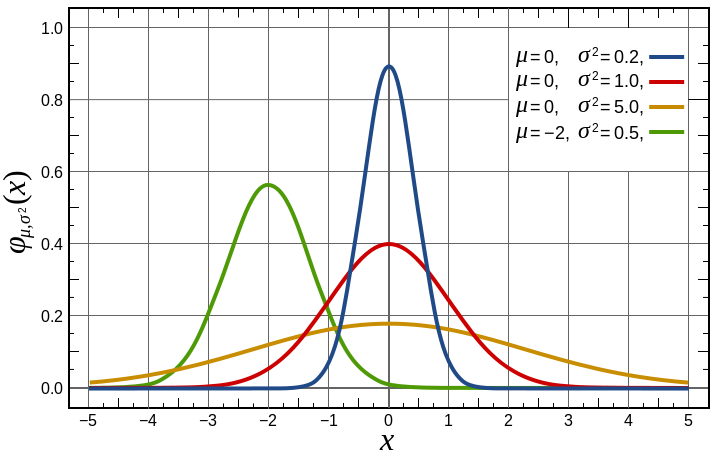
\includegraphics[width=0.7\textwidth]{images/plots/normal_distribution_wikipedia.png}
    \caption{Wikipedia, public domain}
\end{figure}
\end{frame}

%%%%%%%%%%%%%%%%%%%%%%%%%%%%%%%%%%%%%%%%%%%%%%%%%%%%%%%%%%%%%%%%%%%%%%%%%

\begin{frame}
\begin{block}{The multivariate Gaussian (in N dimensions)}
\[f(\bx) = \frac{1}{(2\pi)^{N/2}|\bSigma|^{1/2}} \exp \left(-\frac{1}{2} (\bx-\bmu)\transpose \bSigma\inv (\bx-\bmu) \right)\]
\begin{itemize}
\item $\bx$ and $\bmu$ are $N\times 1$ (column) vectors
\item $\bSigma$ is an $N\times N$ matrix
\end{itemize}
\end{block}

An example in 2 dimensions:
\begin{columns}[T]
\begin{column}{.3\textwidth}
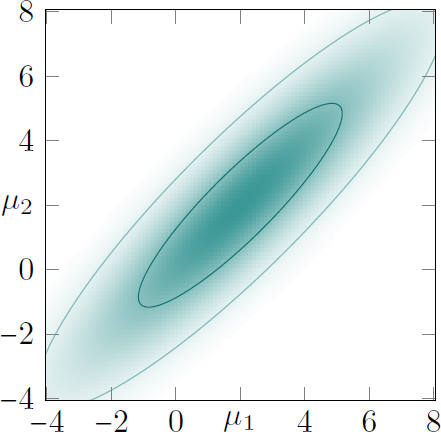
\includegraphics[width=\textwidth]{images/plots/Gaussian-2d.png}
\end{column}
\begin{column}{.5\textwidth}
\vspace*{1cm}
$\bmu =
\begin{pmatrix}
\mu_1\\
\mu_2
\end{pmatrix}
\;\;\;\;\;\;
\bSigma = 
\begin{pmatrix}
\sigma^2_{11}\;\;\sigma^2_{12}\\
\sigma^2_{21}\;\;\sigma^2_{22}\\
\end{pmatrix}
$
\end{column}

\end{columns}
\end{frame}

%%%%%%%%%%%%%%%%%%%%%%%%%%%%%%%%%%%%%%%%%%%%%%%%%%%%%%%%%%%%%%%%%%%%%%%%%

\begin{frame}
\frametitle{Property 1: Closure under marginalization}

\begin{block}{Gaussian distributions are closed under marginalization}
Let $\bx_1$ and $\bx_2$ be jointly Gaussian distributed:
$\bmu =
\begin{bmatrix}
\bx_1\\
\bx_2
\end{bmatrix}
\sim \norm\left(
\begin{bmatrix}
\bmu_1\\
\bmu_2
\end{bmatrix},
\begin{bmatrix}
\bSigma_{11} & \bSigma_{12}\\
\bSigma_{12}\transpose & \bSigma_{22}
\end{bmatrix}
\right)$
\vspace*{0.3cm}
Then $x \sim \norm(\mu_1, \bSigma_{11})$.
\end{block}

%An example in 2 dimensions:
\begin{columns}[T]
\begin{column}{.3\textwidth}
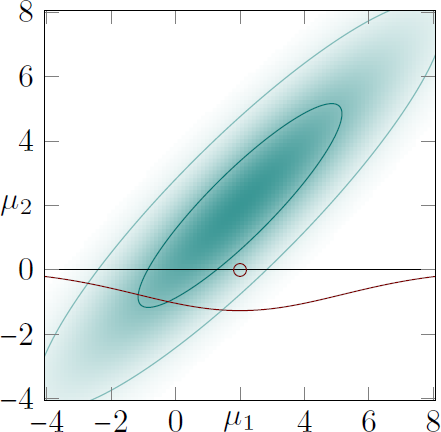
\includegraphics[width=\textwidth]{images/plots/Gaussian-2d-marginalization.png}
\end{column}
\begin{column}{.5\textwidth}
\vspace*{1cm}
$\bmu =
\begin{pmatrix}
\mu_1\\
\mu_2
\end{pmatrix}
\;\;\;\;\;\;
\bSigma = 
\begin{pmatrix}
\sigma^2_{11}\;\;\sigma^2_{12}\\
\sigma^2_{21}\;\;\sigma^2_{22}\\
\end{pmatrix}
$
\end{column}

\end{columns}
\end{frame}

%%%%%%%%%%%%%%%%%%%%%%%%%%%%%%%%%%%%%%%%%%%%%%%%%%%%%%%%%%%%%%%%%%%%%%%%%

\begin{frame}
\frametitle{Property 2: Closure under conditioning}

\begin{block}{Gaussian distributions are closed under conditioning}
Let $\ba$ and $\bb$ be jointly Gaussian distributed:
\vspace*{0.1cm}
$\begin{bmatrix}
\ba\\
\bb
\end{bmatrix}
\sim \norm\left(
\begin{bmatrix}
\bmu_a\\
\bmu_b
\end{bmatrix},
\begin{bmatrix}
A & C\\
C\transpose & B
\end{bmatrix}
\right)$\\
\vspace*{0.1cm}
Then $\bb | \ba \sim \norm\left( \bmu_b + C\transpose A\inv (\ba-\mu_a), B - C\transpose{} A\inv{} C \right)$.
\end{block}

%An example in 2 dimensions:\\
\centering
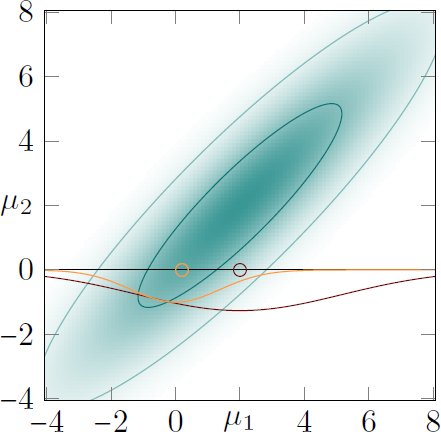
\includegraphics[width=0.3\textwidth]{images/plots/Gaussian-2d-conditioning}

\end{frame}

%%%%%%%%%%%%%%%%%%%%%%%%%%%%%%%%%%%%%%%%%%%%%%%%%%%%%%%%%%%%%%%%%%%%%%%%%

\begin{frame}
\frametitle{Property 3: Closure under multiplication}

%\vspace*{-2cm}
\begin{overlayarea}{\textwidth}{.45\textheight}
  \centering
  \only<1>{\color{green}{$\norm(x; a, A)$} \\~\\~\\
           \vspace*{0.5cm}
           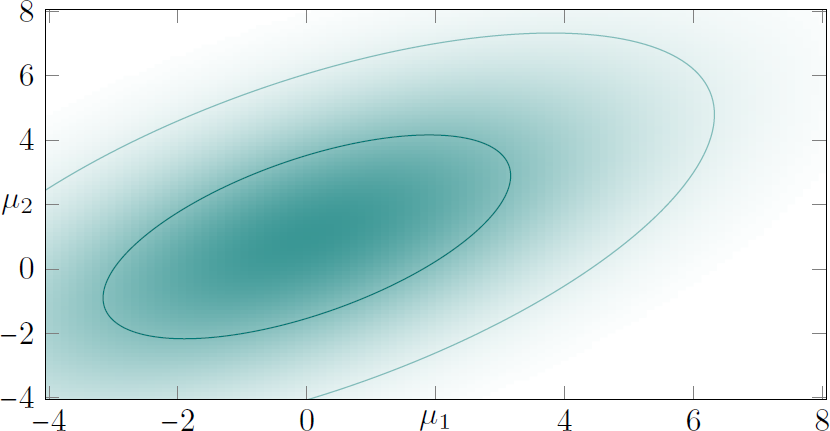
\includegraphics[width=0.7\textwidth]{images/plots/Gaussian-prior.png}}
  \only<2>{
           \color{blue}{$\norm(x; b, B)$} \\~\\~\\
           \vspace*{0.5cm}
           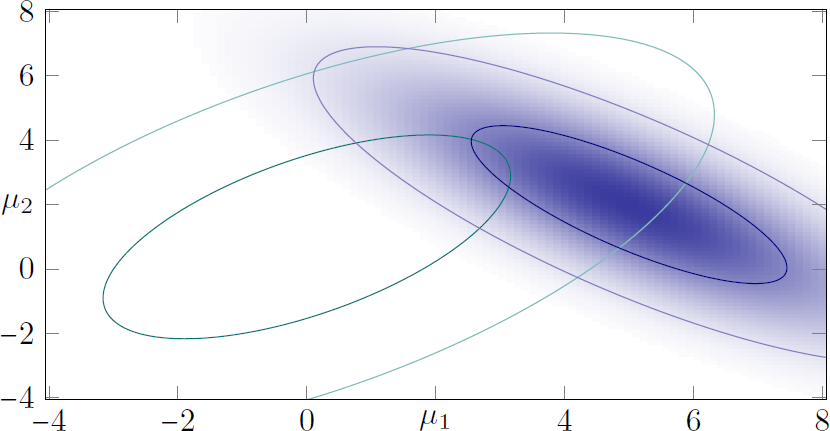
\includegraphics[width=0.7\textwidth]{images/plots/Gaussian-likelihood.png}}
  \only<3>{
            \color{green}{$\norm(x; a, A)$}\color{blue}{$\norm(x; b, B)$}  \color{black}{$\propto$} \color{red}{$\norm(x; c, C)$} \\~\\
            \color{red}{$C:= (A^{-1} + B^{-1})^{-1}~~~c:=C(A^{-1}a+B^{-1}b)$} \\
            \vspace*{0.5cm}
            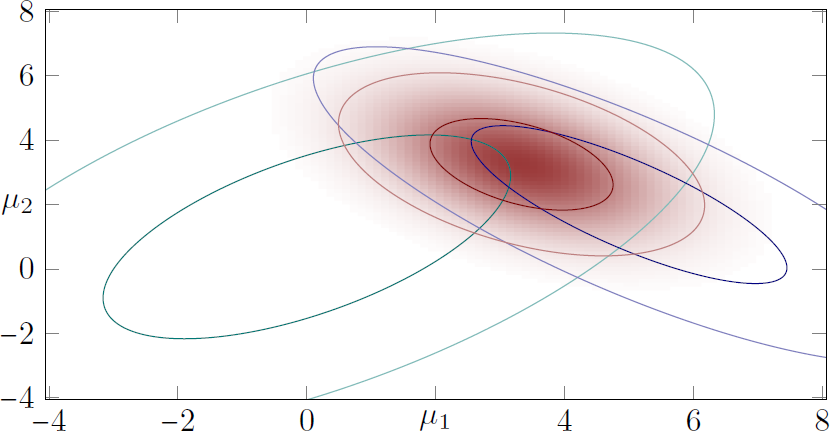
\includegraphics[width=0.7\textwidth]{images/plots/Picture-posterior.png}}
\end{overlayarea}
\end{frame}


%%%%%%%%%%%%%%%%%%%%%%%%%%%%%%%%%%%%%%%%%%%%%%%%%%%%%%%%%%%%%%%%%%%%%%%%%

\begin{frame}
\frametitle{Why Gaussians?}
\begin{itemize}
\item The central limit theorem tells us that means of large
populations are distributed according to a Gaussian
\item However, individual measurements are very rarely
Gaussian-distributed
\item Rather, Gaussians are mostly a mathematical
convenience that lets us solve integrals in closed form!
\end{itemize}
\end{frame}

%%%%%%%%%%%%%%%%%%%%%%%%%%%%%%%%%%%%%%%%%%%%%%%%%%%%%%%%%%%%%%%%%%%%%%%%%

\section{Gaussian processes: the weight space view}
\subsection{Bayesian linear regression}
\begin{frame}
\frametitle{Regression}
\begin{figure}
    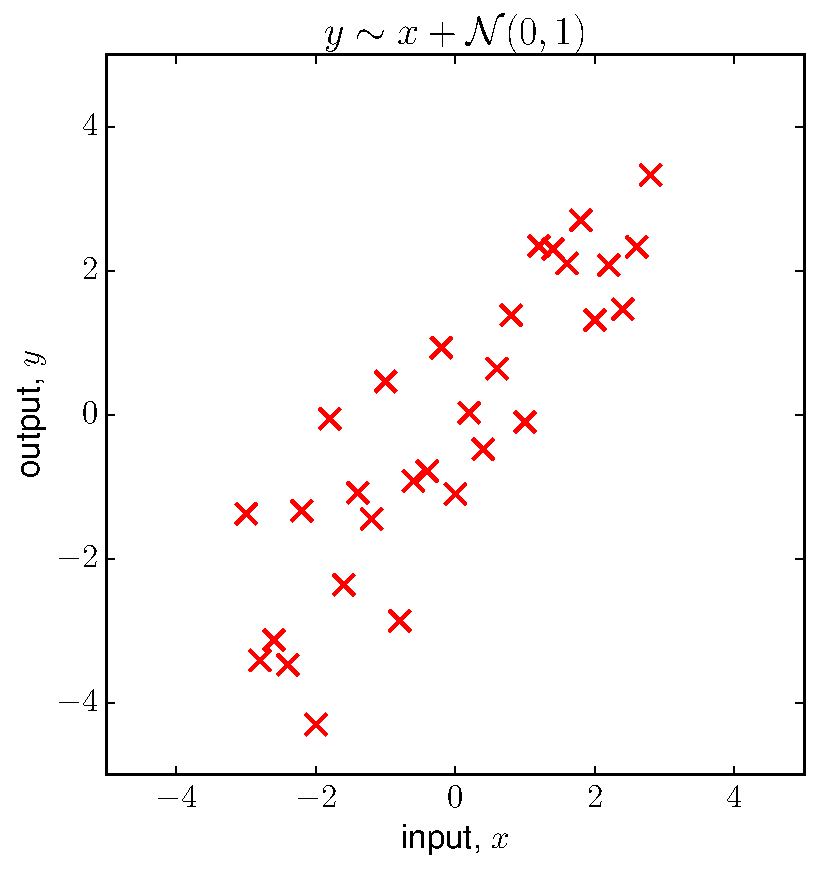
\includegraphics[width=0.25\textwidth]{images/plots/w_space_maximum_likelihood_001.pdf}
\end{figure}
\begin{itemize}
	\item We have a dataset of n i.i.d. observations, $\mathcal{D} = \{(\bm{x}_i, y_i | i = 1, \ldots ,n\}$
	\item Each $\bx_i$ denotes an input (column) vector of dimension $D$ and each $y_i$ is a scalar output or target
	\item We collect all inputs $\bx_i$ into the $D \times n$ design matrix 
	$\bX = [\bx_1 \cdots \bx_n]$  and the targets into the $n \times 1$ vector $\by$.
	\item Note: these slides are using the notation of Rasmussen's and Williams' book; $\bX$ is transposed from our usual use
\end{itemize}
\end{frame}

%%%%%%%%%%%%%%%%%%%%%%%%%%%%%%%%%%%%%%%%%%%%%%%%%%%%%%%%%%%%%%%%%%%%%%%%%

\begin{frame}
\frametitle{Standard Linear Regression Model}
\begin{figure}
    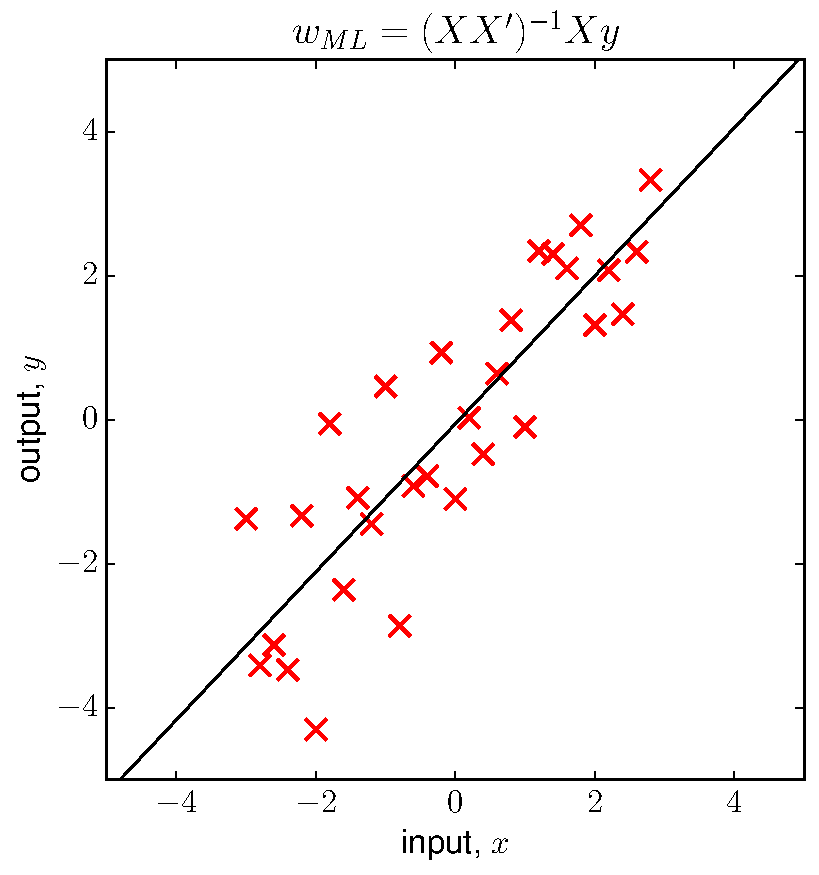
\includegraphics[width=0.3\textwidth]{images/plots/w_space_maximum_likelihood_002.pdf}
\end{figure}

\renewcommand\theequation{2.\thedefcounter}
\setcounter{defcounter}{1}
\begin{equation}
f(\bx) = \bx\transpose \bw,~~~~~y = f(\bx) + \epsilon
\end{equation}

\setcounter{defcounter}{2}
\begin{equation}
\epsilon \sim \norm(0, \sigma_n^2)
\end{equation}

\end{frame}

%%%%%%%%%%%%%%%%%%%%%%%%%%%%%%%%%%%%%%%%%%%%%%%%%%%%%%%%%%%%%%%%%%%%%%%%%

\begin{frame}
\frametitle{The predictive distribution with fixed $\bw$}

\renewcommand\theequation{2.\thedefcounter}
\setcounter{defcounter}{3}
\begin{align}
p(\by | X, \bw) &= \prod_{i=1}^{n} p(y_i | \bx_i, \bw) \nonumber \\
                &= \prod_{i=1}^{n} \frac{1}{(\sqrt{2\pi}\sigma_n)} \exp{\left( -\frac{(y_i - \bx_i\transpose\bw_i)^2}{2 \sigma_n^2} \right) } \nonumber \\
                &= \frac{1}{(2\pi\sigma_n^2)^{n/2}} \exp{\left( -\frac{1}{2\sigma_n^2} | \by - \bX\transpose\bw |^2 \right)} \nonumber \\
                &= \norm(\by; \bX\transpose\bw, \sigma_n^2I)
\end{align}

~\\
How does each of these steps follow? 	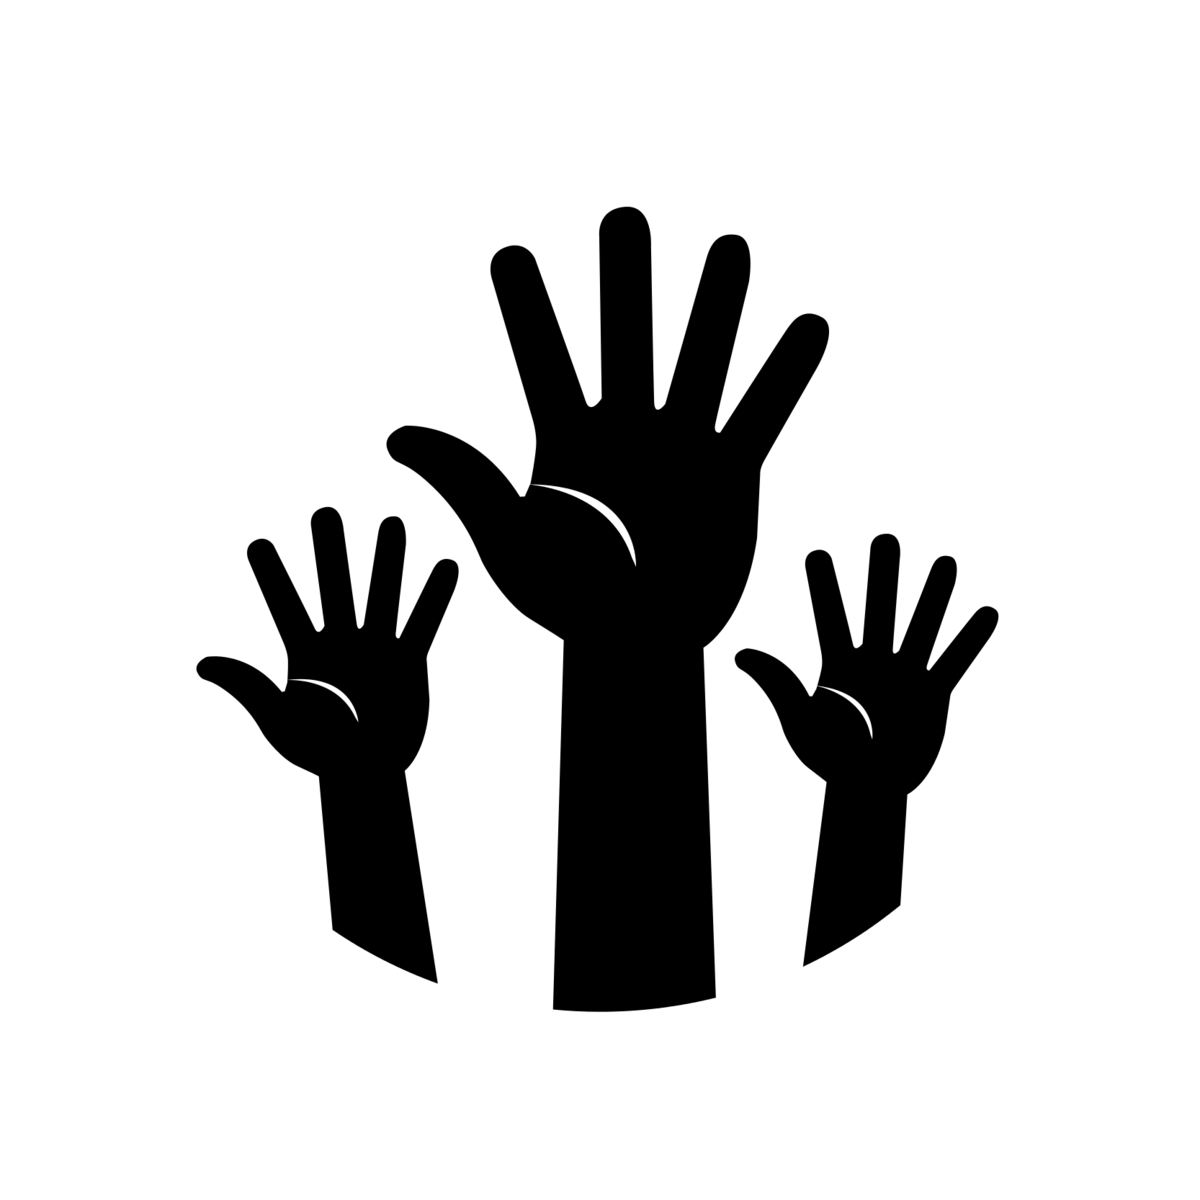
\includegraphics[width=0.1\textwidth]{images/hands.png}

\end{frame}


%%%%%%%%%%%%%%%%%%%%%%%%%%%%%%%%%%%%%%%%%%%%%%%%%%%%%%%%%%%%%%%%%%%%%%%%%

\begin{frame}
\frametitle{The Bayesian way of setting $\bw$}

\begin{itemize}
\item Define a \alert{prior distribution over $\bw$} quantifying our uncertainty
\item Integrate the likelihood $p(\by|\bX,\bw)$ of the training data across all possible values of $\bw$, weighted by the prior $p(\bw)$
\end{itemize}

\renewcommand\theequation{2.\thedefcounter}
\setcounter{defcounter}{6}
\begin{equation}
p(\by|\bX) = \int p(\by|\bX,\bw) p(\bw) d\bw
\label{eq:integrated_likelihood}
\end{equation}

\begin{itemize}
\item \alert{We don't commit to a single $\bw$, but integrate over an infinite number of possibilities}
\end{itemize}

\end{frame}

%%%%%%%%%%%%%%%%%%%%%%%%%%%%%%%%%%%%%%%%%%%%%%%%%%%%%%%%%%%%%%%%%%%%%%%%%

\begin{frame}
\frametitle{The Bayesian way of setting $\bw$}
We combine the prior and the data likelihood using Bayes' rule:
\renewcommand\theequation{2.\thedefcounter}
\setcounter{defcounter}{5}
\begin{equation*}
\text{posterior} = \frac{\text{likelihood} \times \text{prior}}{\text{marginal likelihood}}
\end{equation*}

\begin{equation}
p(\bw|\by, \bX) = \frac{p(\by|\bX, \bw)p(\bw)}{p(\by|\bX)}
\end{equation}

\begin{figure}
\begin{tabular}{ccc}
    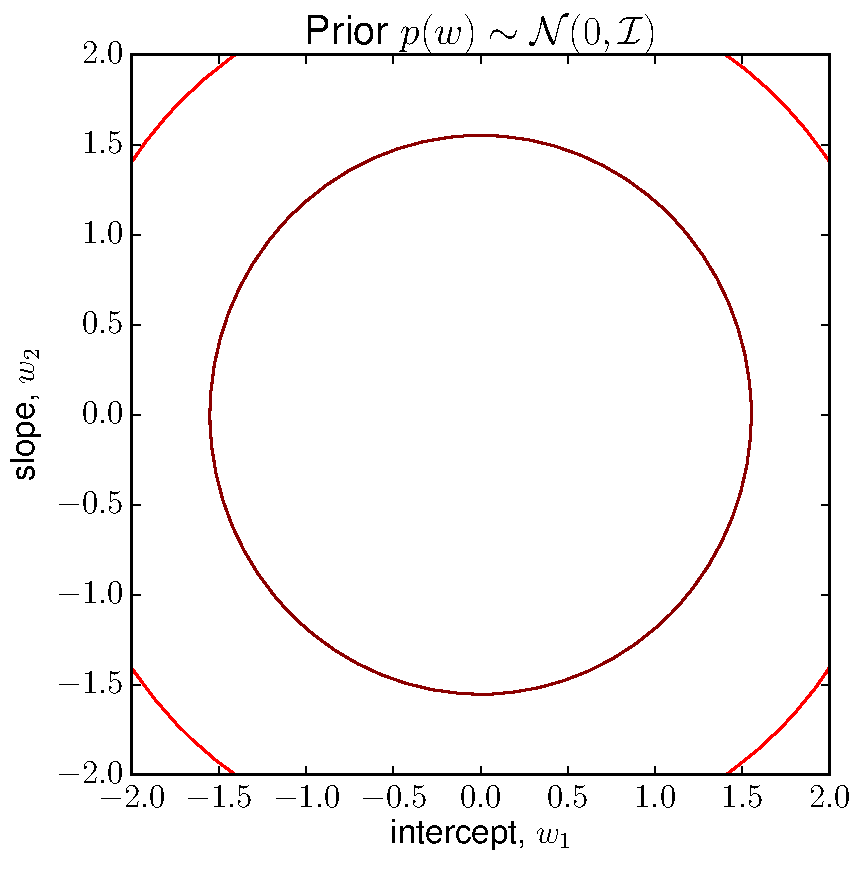
\includegraphics[width=0.3\textwidth]{images/plots/w_space_prior.pdf} &
    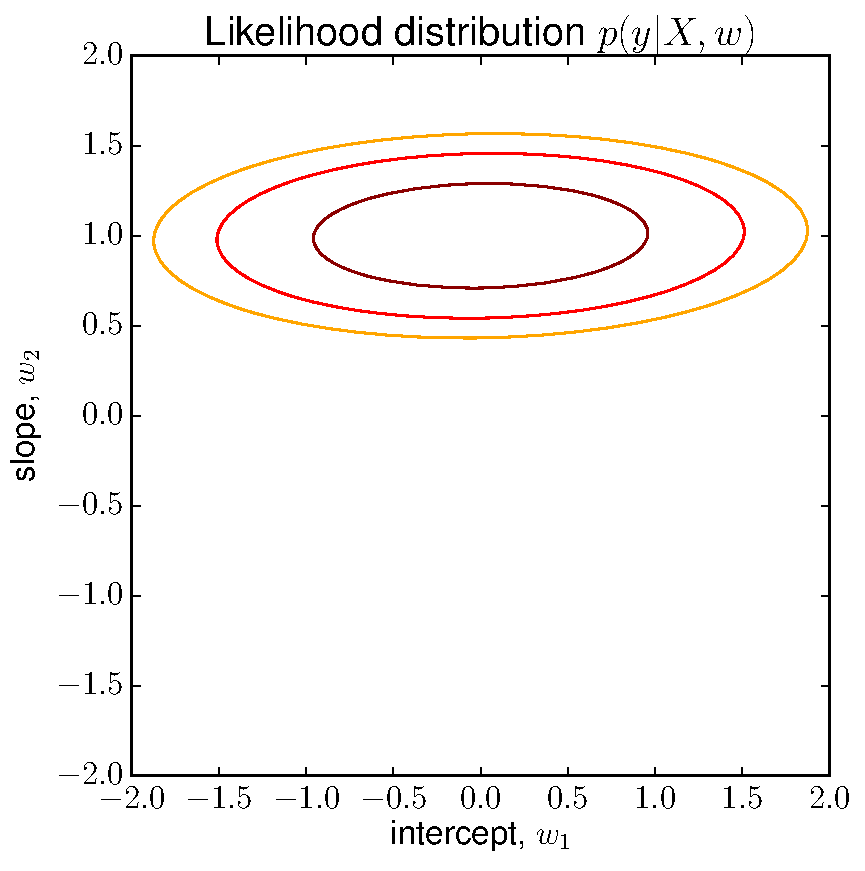
\includegraphics[width=0.3\textwidth]{images/plots/w_space_likelihood.pdf} &
    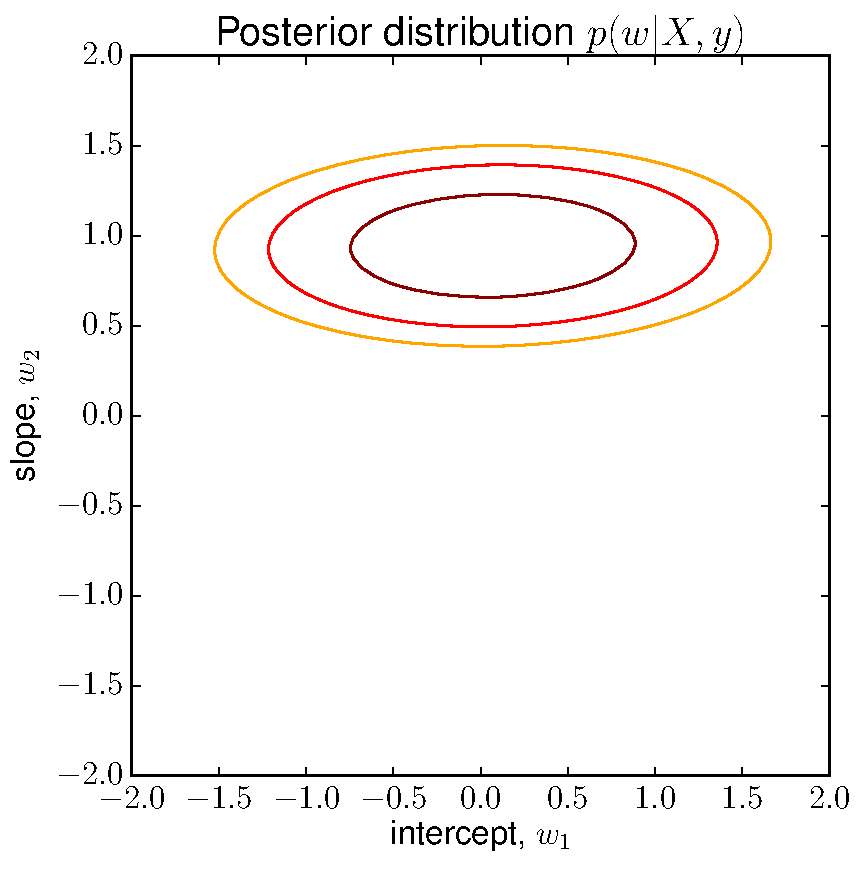
\includegraphics[width=0.3\textwidth]{images/plots/w_space_posterior.pdf} \\
\end{tabular}
\end{figure}

\end{frame}

%%%%%%%%%%%%%%%%%%%%%%%%%%%%%%%%%%%%%%%%%%%%%%%%%%%%%%%%%%%%%%%%%%%%%%%%%

\begin{frame}
\frametitle{Posterior of $\bw$ under a Gaussian prior on $\bw$}

In general, the posterior $p(\bw|\bX, \by)$ has no closed-form solution, but 
%Equation \eqref{eq:integrated_likelihood} generally requires approximating a complicated integral, but 
it simplifies if we choose a prior $p(\bw)$ that is \textcolor{red}{conjugate} to the likelihood; in this case another Gaussian:

\renewcommand\theequation{2.\thedefcounter}
\setcounter{defcounter}{4}
\begin{equation}
\bw \sim \norm(0, \Sigma_p)
\end{equation}

In that case, the posterior is Gaussian again:
\setcounter{defcounter}{7}
\begin{equation}
p(\bw|\bX, \by) \sim \norm\left(\bar{\bw} = \frac{1}{\sigma_n^2}A\inv \bX\by, A\inv\right)
\label{eq:posterior_2_7},
\end{equation}

with $A = \frac{1}{\sigma_n^2} \bX \bX\transpose + \Sigma_p^{-1}$.\\~\\

We'll do the core of the derivation for this on the next two slides.

%\alert{You will derive this identity be part of this week's exercise.}

%The derivation of this equation uses the trick of \textit{completing the square} \alert{$\rightarrow$ you'll do this in the exercise}

\end{frame}

%%%%%%%%%%%%%%%%%%%%%%%%%%%%%%%%%%%%%%%%%%%%%%%%%%%%%%%%%%%%%%%%%%%%%%%%%
%
%\begin{frame}
%\frametitle{\textit{Completing the square}}
%
%
%The derivation uses the \alert{trick of \emph{completing the square}.}
%
%\vspace*{-0.1cm}
%\begin{itemize}
%  \item The data likelihood is $p(\by | \bX, \bw) = \norm(\by; \bX\transpose{}\bw, \sigma^2_n \bI)$.
%  \item Written as a function of $\bw$, this turns out to be proportional to a Gaussian $\mathcal{L}(w; \by, \bX) = p(\by | \bX, \bw) \propto \norm( \bw; \bm{w'}, \bSigma\inv )$
%  \item We show this by matching coefficients of $\bw$ and $\bw\transpose \bw$.
%\end{itemize}
%\pause
%
%\vspace*{0.5cm}
%Thus, the posterior $p(\bw|\by, \bX) = \frac{p(\by|\bX, \bw)p(\bw)}{p(\by|\bX)}$ is a Gaussian.
%


%\begin{eqnarray}
%\nonumber{}\mathcal{L}(w; \by, \bX) & \propto \exp \left(-\frac{1}{2 \sigma^2_n} \left(\by\transpose\by - 2 \bw\transpose\bX\by + (\bX\transpose\bw)\transpose \bX\transpose\bw \right) \right)
%\end{eqnarray}

%\end{frame}


%%%%%%%%%%%%%%%%%%%%%%%%%%%%%%%%%%%%%%%%%%%%%%%%%%%%%%%%%%%%%%%%%%%%%%%%%

%%%%%%%%%%%%%%%%%%%%%%%%%%%%%%%%%%%%%%%%%%%%%%%%%%%%%%%%%%%%%%%%%%%%%%%%%


\begin{frame}
\frametitle{Key part of the derivation: completing the square (1)}
%
\vspace*{-0.1cm}
\begin{itemize}
  \item The data likelihood is $p(\by | \bX, \bw) = \norm(\by; \bX\transpose{}\bw, \sigma^2_n \bI)$.
  \item Written as a function of $\bw$, this turns out to be proportional to a Gaussian $\mathcal{L}(w; \by, \bX) = p(\by | \bX, \bw) \propto \norm( \bw; \bm{w'}, \bSigma )$
  \item We show this by matching coefficients of $\bw$ and $\bw\transpose \bw$.
\end{itemize}
\pause
%
\vspace*{-0.2cm}
%
\begin{align*}
\mathcal{L}(w; \by, \bX)~=~& \frac{1}{(2\pi\sigma^2_n)^{n/2}} \exp \left(-\frac{1}{2 \sigma^2_n} (\by-\bX\transpose\bw)\transpose (\by-\bX\transpose\bw) \right) \\
                         \propto~& \exp \left(-\frac{1}{2 \sigma^2_n} (\by-\bX\transpose\bw)\transpose (\by-\bX\transpose\bw) \right) \\
                         =~& \exp \left(-\frac{1}{2 \sigma^2_n} \left(\by\transpose\by - 2 \bw\transpose\bX\by + (\bX\transpose\bw)\transpose \bX\transpose\bw \right) \right)
\end{align*}
%
\vspace*{-0.5cm}
%
\pause
\begin{align*}
p(\bw | \bm{w'}, \bSigma)~=~& \frac{1}{(2\pi)^{n/2}|\bSigma|^{1/2}} \exp \left(-\frac{1}{2} (\bw-\bm{w'})\transpose \bSigma^{-1} (\bw-\bm{w'}) \right) \\
\propto~& \exp \left( -\frac{1}{2} \left( \bw \transpose \bSigma\inv \bw -2 \bw\transpose \bSigma\inv \bm{w'} + {\bm{w'}}\transpose \bSigma\inv \bm{w'} \right) \right)
\end{align*}
%
\vspace*{-0.3cm}
%
\end{frame}

%%%%%%%%%%%%%%%%%%%%%%%%%%%%%%%%%%%%%%%%%%%%%%%%%%%%%%%%%%%%%%%%%%%%%%%%%
\begin{frame}
\frametitle{Key part of the derivation: completing the square (2)}

Let's match the coefficients of $\bw$ and $\bw \transpose \bw$\ldots

\vspace*{-0.4cm}

\begin{eqnarray}
\nonumber{}\mathcal{L}(\bw; \by, \bX) & \propto \exp \left(-\frac{1}{2 \sigma^2_n} \left(\by\transpose\by - 2 \bw\transpose\bX\by + (\bX\transpose\bw)\transpose \bX\transpose\bw \right) \right)
\end{eqnarray}

\vspace*{0.1cm}
\begin{eqnarray}
\nonumber{}p(\bw | \bm{w'}, \bSigma) & \propto &  \exp \left(-\frac{1}{2} 
(
\bw\transpose\bSigma\inv{}\bw 
-2\bw\transpose \bSigma\inv{}\bm{w'} + 
{\bm{w'}}\transpose \bSigma^{-1} \bm{w'} 
)
\right)
\end{eqnarray}

\pause
This directly yields: 
\begin{eqnarray}
\nonumber
\bw' & = & \frac{1}{\sigma^2_n} \bSigma \bX \by\\
\nonumber \bSigma & = & \left(\frac{1}{\sigma^2_n} \bX \bX^\transpose{}\right)\inv{}
\end{eqnarray}

\pause

Thus: $\nonumber{}\mathcal{L}(\bw; \by, \bX) \propto \norm \left( \frac{1}{\sigma_n^2} (\frac{1}{\sigma_n^2} \bX \bX\transpose )\inv \bX \by , (\frac{1}{\sigma_n^2} \bX \bX\transpose)\inv\right)$.\\
Then, simply multiply two Gaussians to get the posterior~in~\eqref{eq:posterior_2_7}
\end{frame}


%%%%%%%%%%%%%%%%%%%%%%%%%%%%%%%%%%%%%%%%%%%%%%%%%%%%%%%%%%%%%%%%%%%%%%%%%




\begin{frame}
\frametitle{The posterior predictive distribution}
Recall: in linear regression (so far without basis functions), each weight vector $\bw$ corresponds to a linear model:

\vspace*{-0.2cm}
\renewcommand\theequation{2.\thedefcounter}
\setcounter{defcounter}{1}
\begin{equation}
f(\bx) = \bx\transpose \bw
\end{equation}
\vspace*{0.1cm}

We just derived the posterior $p(\bw|\bX, \by)$ over the weights $\bw$: \renewcommand\theequation{2.\thedefcounter}
\setcounter{defcounter}{7}
\begin{equation}
p(\bw|\bX, \by) \sim \norm\left(\bar{\bw} = \frac{1}{\sigma_n^2}A\inv \bX\by, A\inv\right)
\label{eq:posterior_2_7}.
\end{equation}

\pause
\vspace*{0.3cm}
Gaussians are closed under linear maps. Thus, the posterior predictive distribution at new input $\bx_{\star}$ given training data $\bX$, $\by$ is:
%
\vspace*{-0.3cm}
\renewcommand\theequation{2.\thedefcounter}
\setcounter{defcounter}{9}
\begin{eqnarray}
\label{eq:posterior_pred_dist}
\nonumber{}p(f_{\star} |\bx_{\star}, \bX, \by)
& = & p(\bx_{\star}\transpose \bw|\bX, \by)\\
& = & \norm(f_{\star}; \frac{1}{\sigma_n^2} \bx_{\star}\transpose A\inv \bX \by,
\bx_{\star}\transpose A\inv \bx_{\star} )
%
%\nonumber{}p(f_{\star} |\bx_{\star}, \bX, \by) &= & \int{p(f_{\star} | \bx_{\star}, \bw) p(\bw | \bX, \by)
%d\bw}\\
%                        &= & \norm(f_{\star}; \frac{1}{\sigma_n^2} \bx_{\star}\transpose A\inv \bX \by,
%                         \bx_{\star}\transpose A\inv \bx_{\star} )
\end{eqnarray}

%We simply average the predictions $p(f_{\star} | \bx_{\star}, \bw)$ of linear models with all possible $\bw$, weighting each model by the posterior probability of its corresponding $w$
%

\end{frame}

%%%%%%%%%%%%%%%%%%%%%%%%%%%%%%%%%%%%%%%%%%%%%%%%%%%%%%%%%%%%%%%%%%%%%%%%%

\begin{frame}
\frametitle{Weights correspond to functions (1)}
\begin{figure}
\begin{tabular}{cc}
    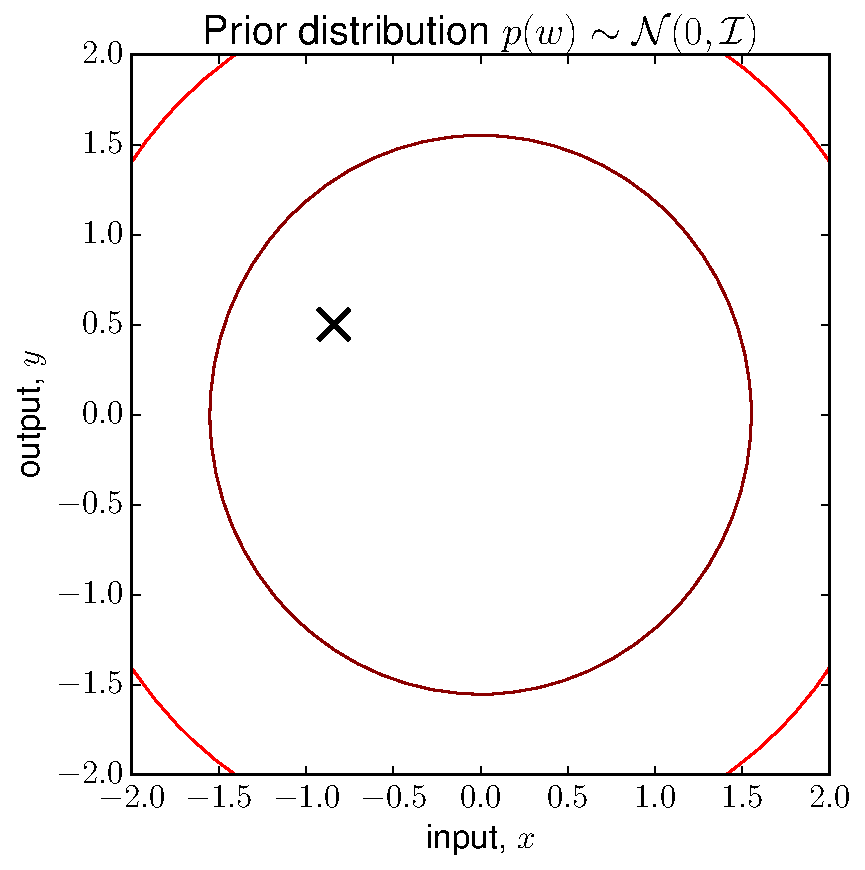
\includegraphics[width=0.3\textwidth]{images/plots/w_space_prior_sequence_001_prior.pdf} &
    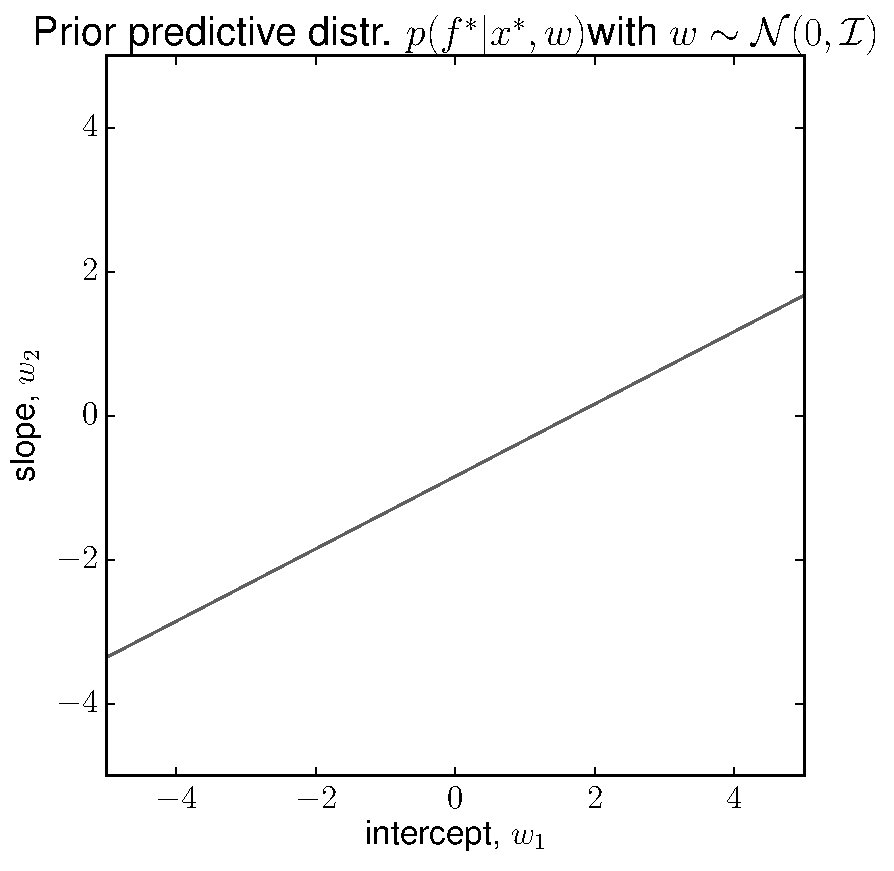
\includegraphics[width=0.3\textwidth]{images/plots/w_space_prior_sequence_001_functions.pdf} \\
    
    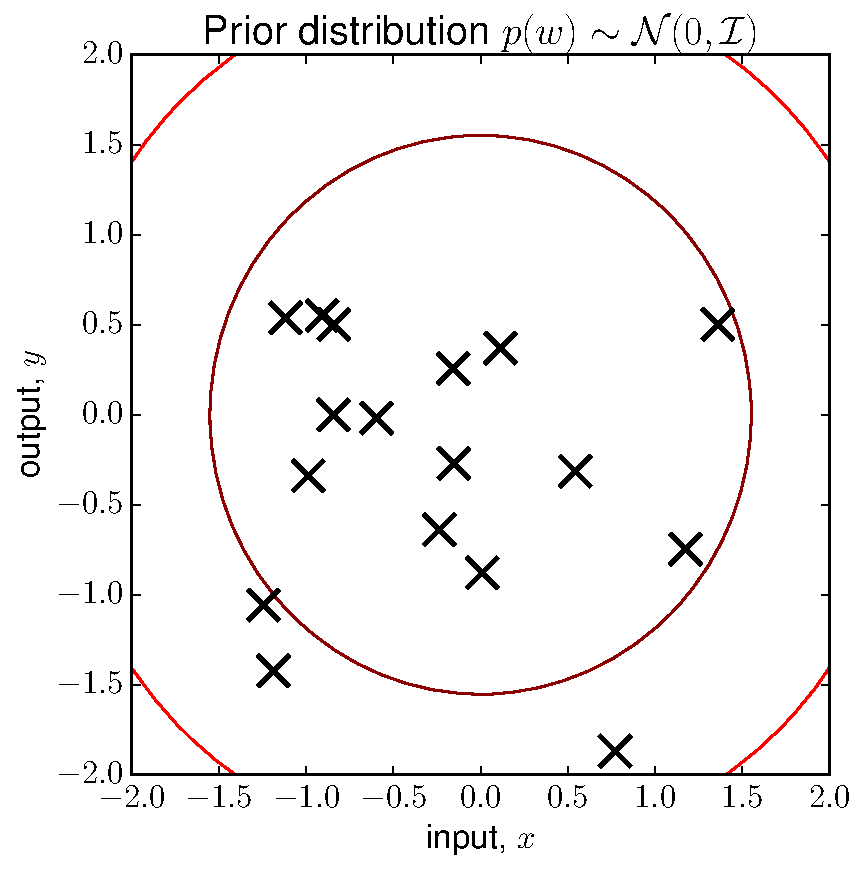
\includegraphics[width=0.3\textwidth]{images/plots/w_space_prior_sequence_019_prior.pdf} &
    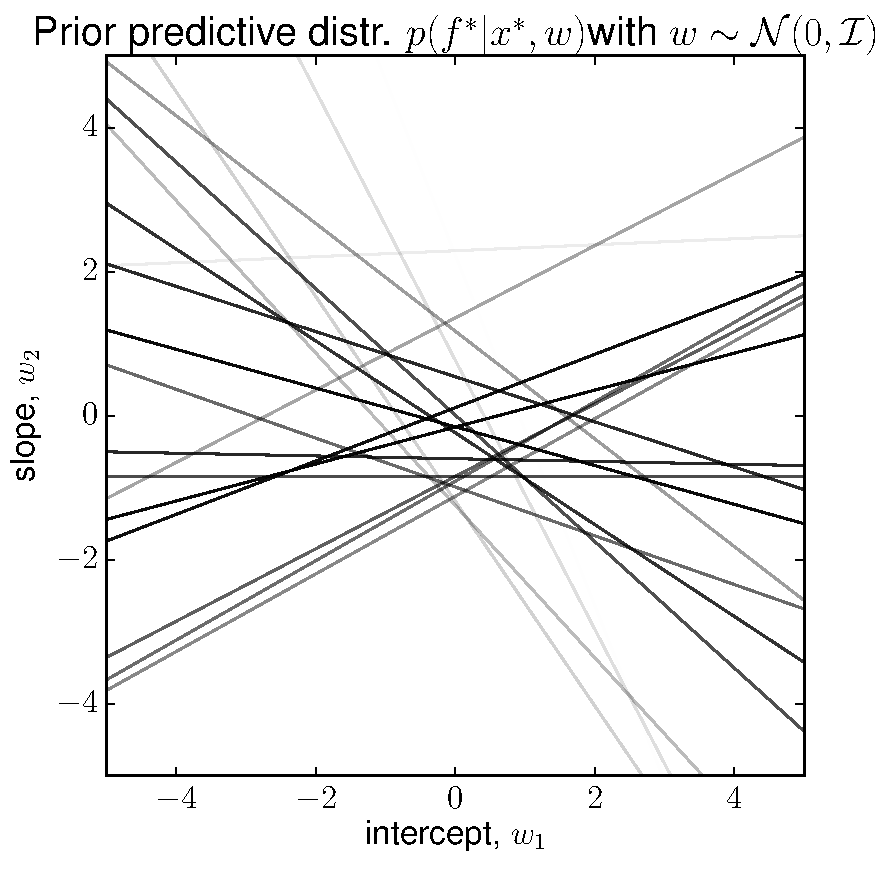
\includegraphics[width=0.3\textwidth]{images/plots/w_space_prior_sequence_019_functions.pdf}
\end{tabular}
\end{figure}
\end{frame}

%%%%%%%%%%%%%%%%%%%%%%%%%%%%%%%%%%%%%%%%%%%%%%%%%%%%%%%%%%%%%%%%%%%%%%%%%

\begin{frame}
\frametitle{Weights correspond to functions (2)}
\begin{figure}
\begin{tabular}{ccc}
    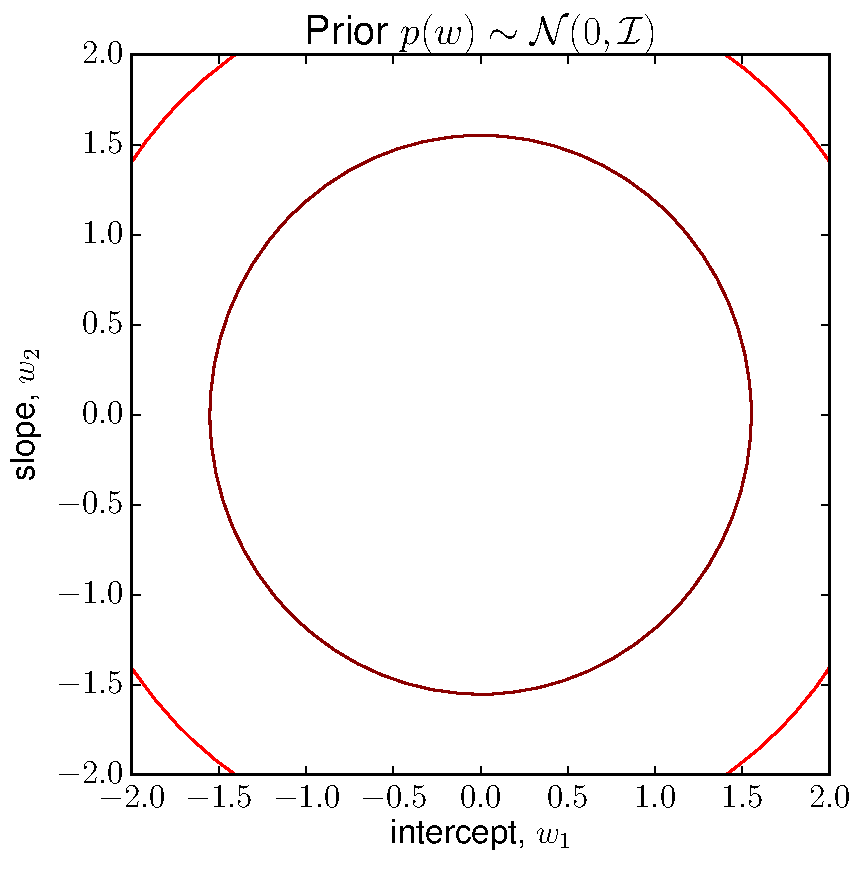
\includegraphics[width=0.3\textwidth]{images/plots/w_space_prior.pdf} &
    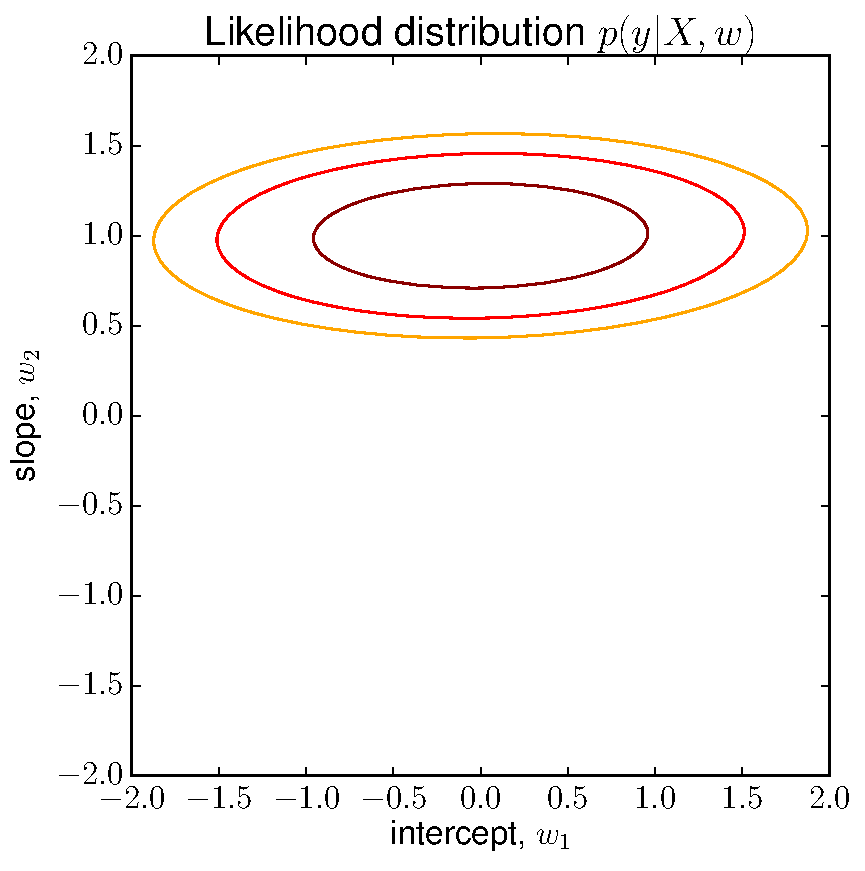
\includegraphics[width=0.3\textwidth]{images/plots/w_space_likelihood.pdf} &
    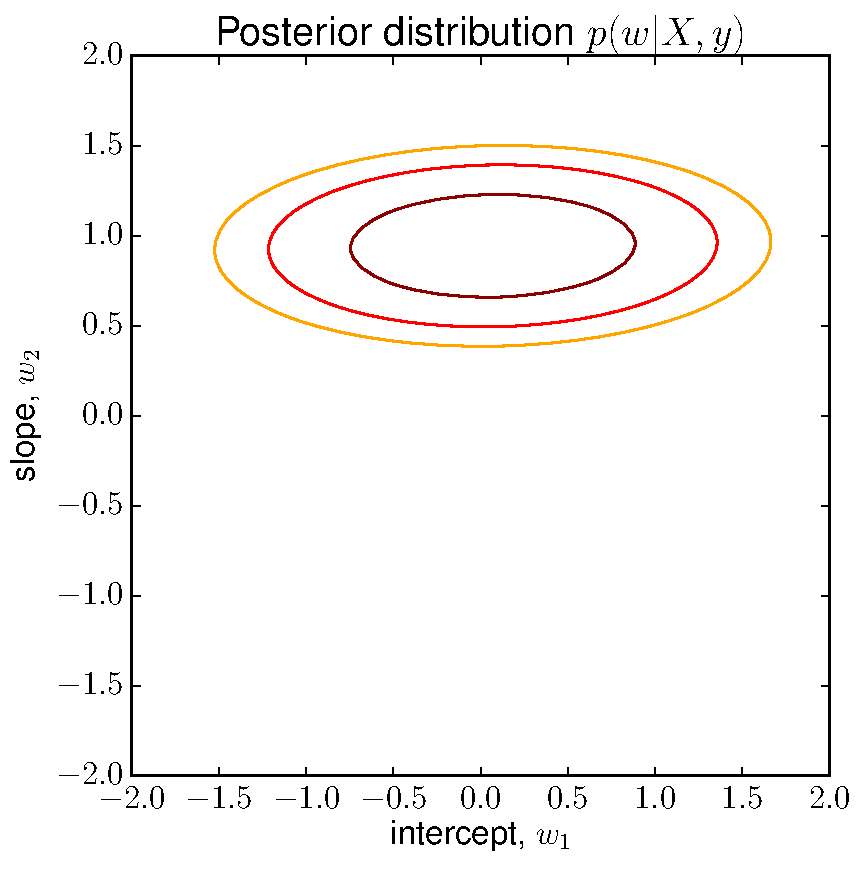
\includegraphics[width=0.3\textwidth]{images/plots/w_space_posterior.pdf} \\

    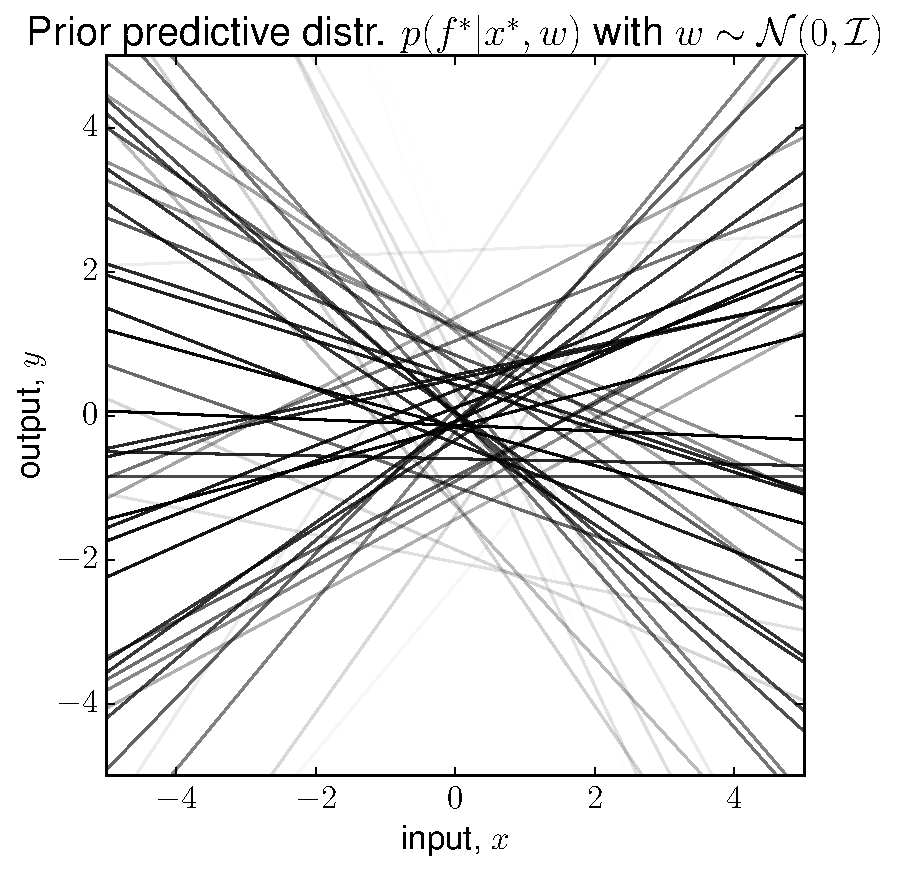
\includegraphics[width=0.3\textwidth]{images/plots/w_space_prior_models.pdf} & &
    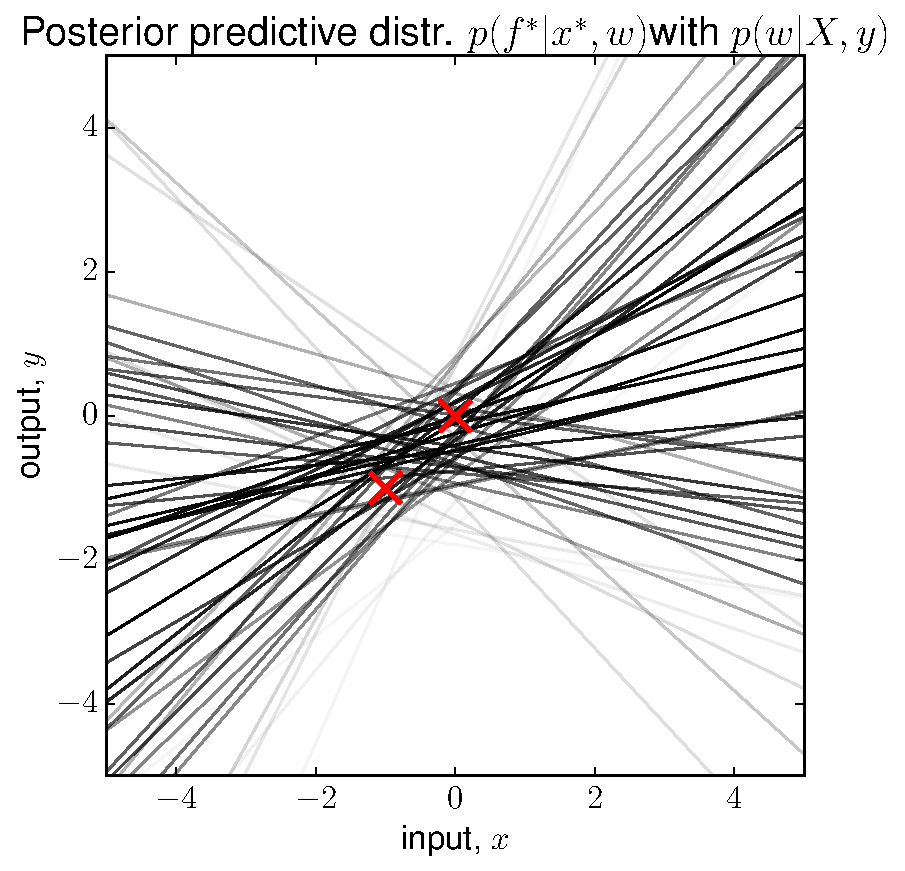
\includegraphics[width=0.3\textwidth]{images/plots/w_space_posterior_sequence_002_posterior_models.pdf} \\
\end{tabular}
\end{figure}
\end{frame}

%%%%%%%%%%%%%%%%%%%%%%%%%%%%%%%%%%%%%%%%%%%%%%%%%%%%%%%%%%%%%%%%%%%%%%%%%

\begin{frame}
\frametitle{Enough data overwhelms the prior}
\vspace*{-0.2cm}
\begin{figure}
\begin{tabular}{ccc}
    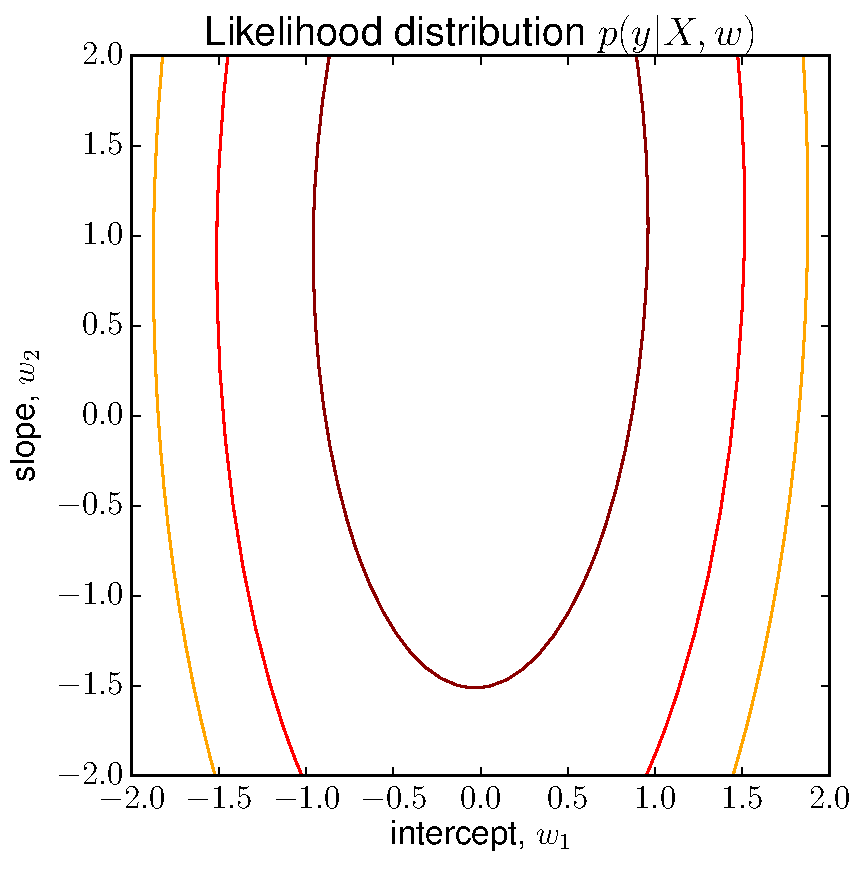
\includegraphics[width=0.3\textwidth]{images/plots/w_space_posterior_sequence_002_likelihood.pdf} &
    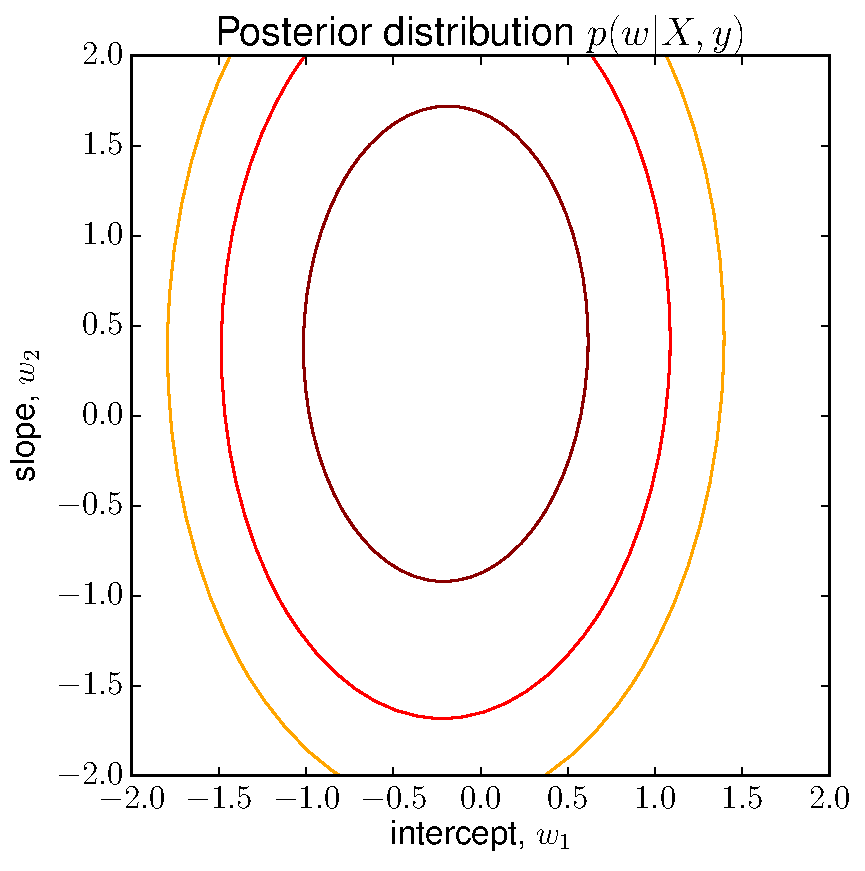
\includegraphics[width=0.3\textwidth]{images/plots/w_space_posterior_sequence_002_posterior.pdf} &
    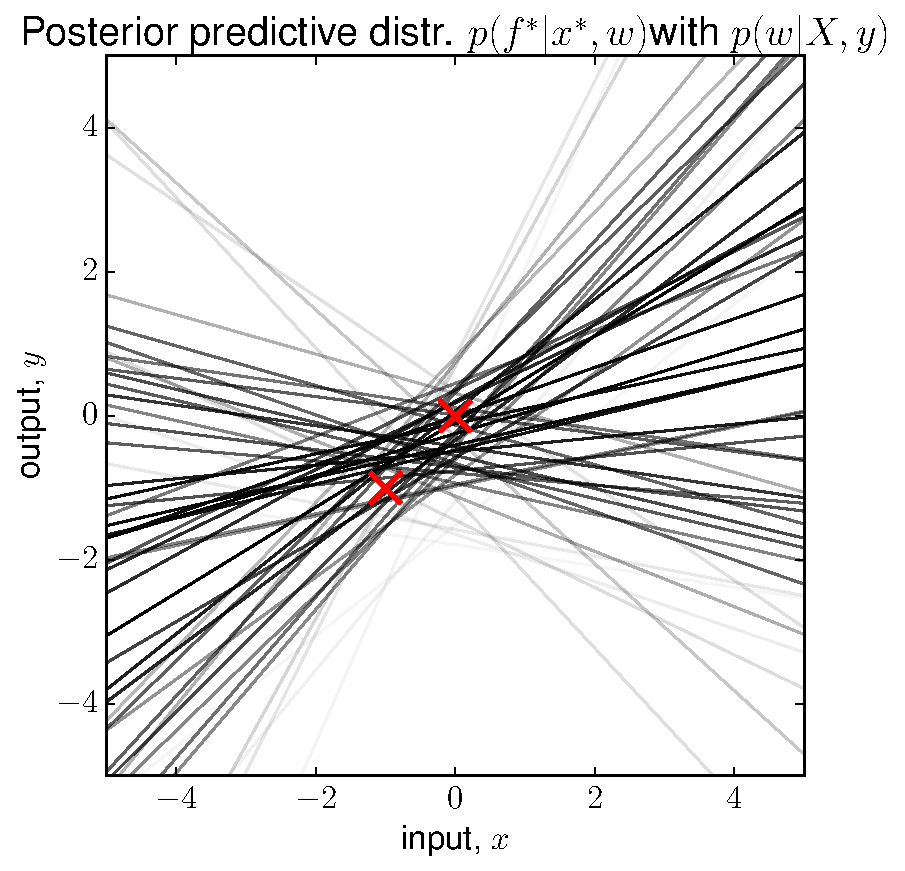
\includegraphics[width=0.3\textwidth]{images/plots/w_space_posterior_sequence_002_posterior_models.pdf} \\ 
    
    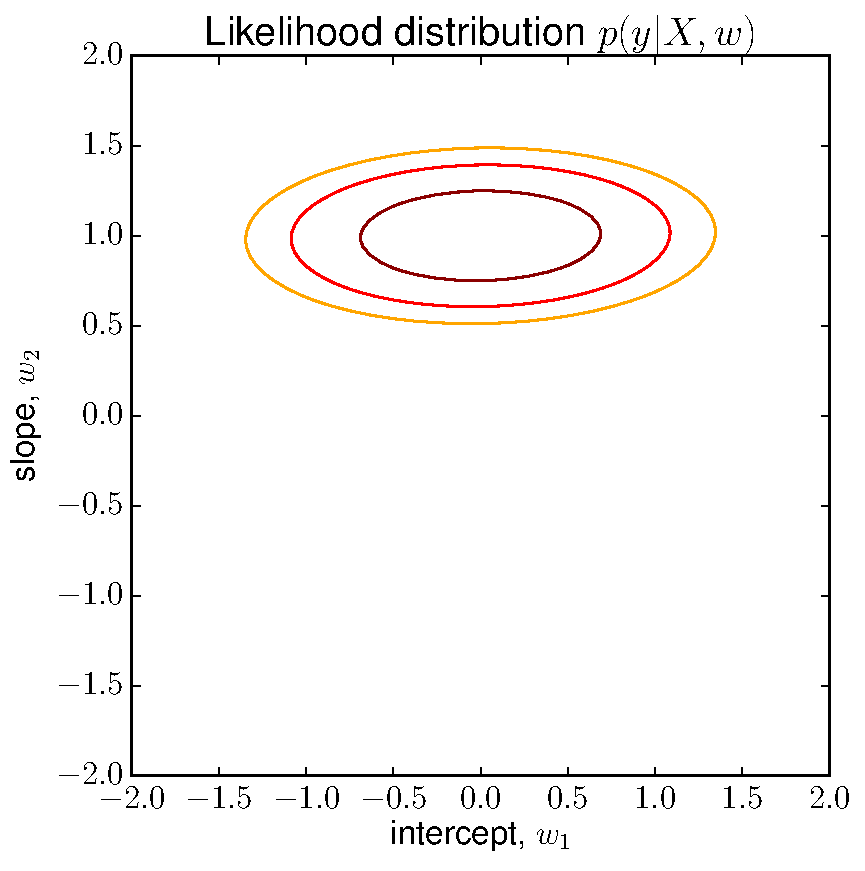
\includegraphics[width=0.3\textwidth]{images/plots/w_space_posterior_sequence_006_likelihood.pdf} &
    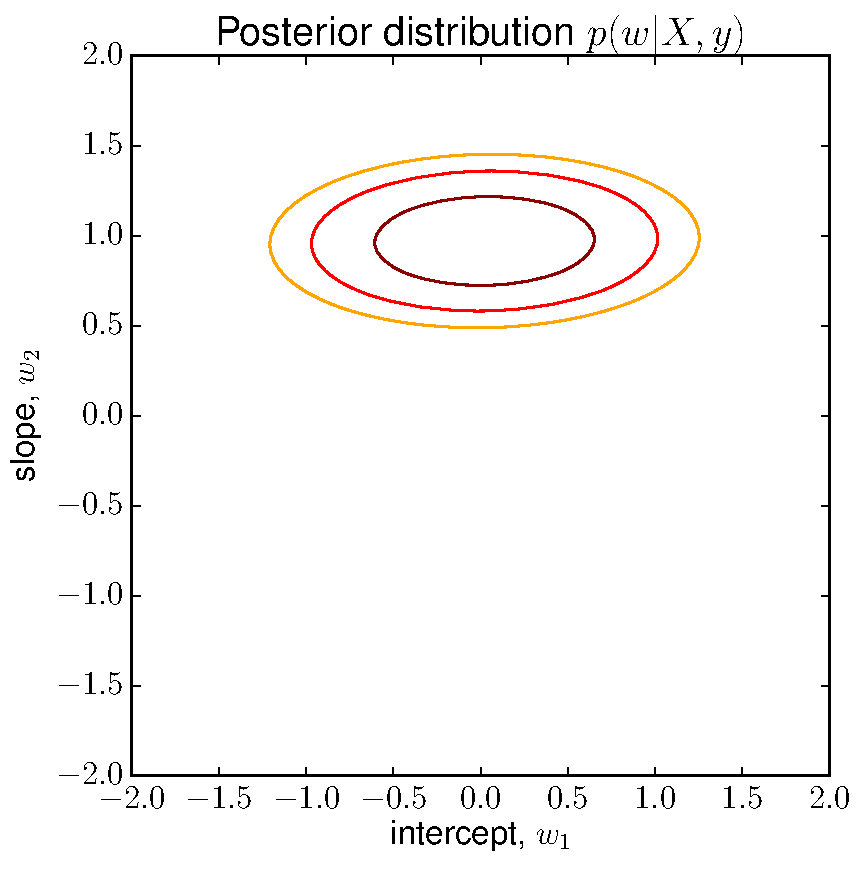
\includegraphics[width=0.3\textwidth]{images/plots/w_space_posterior_sequence_006_posterior.pdf} &
    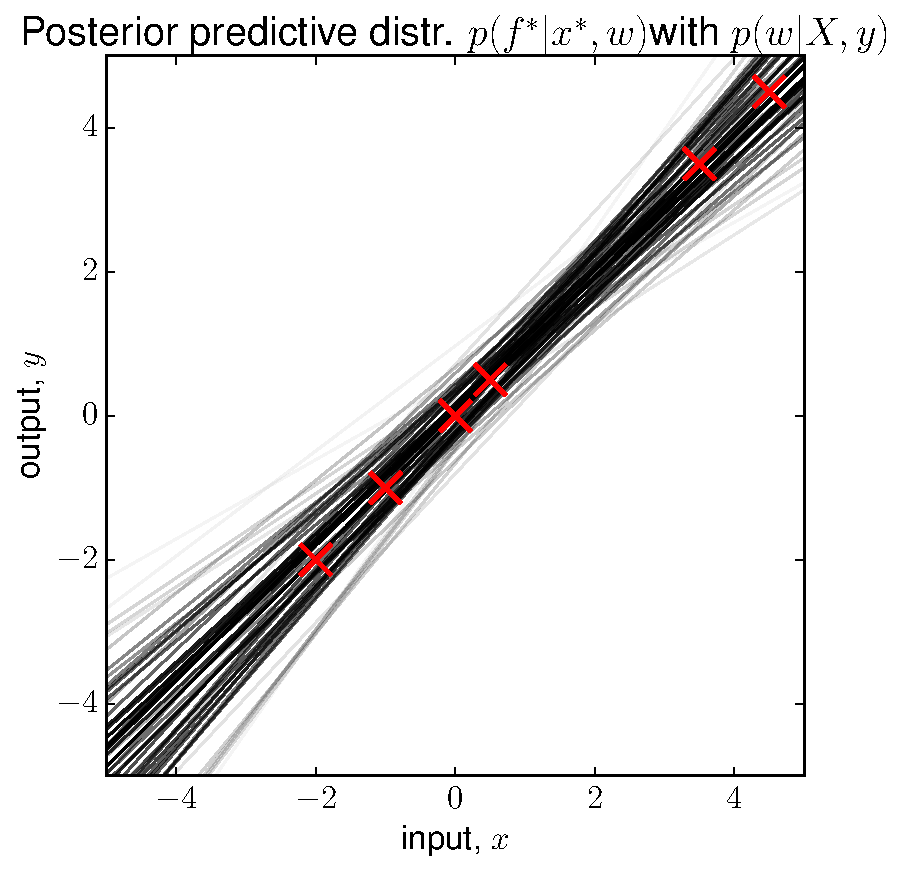
\includegraphics[width=0.3\textwidth]{images/plots/w_space_posterior_sequence_006_posterior_models.pdf}
\end{tabular}
\end{figure}
\end{frame}

%%%%%%%%%%%%%%%%%%%%%%%%%%%%%%%%%%%%%%%%%%%%%%%%%%%%%%%%%%%%%%%%%%%%%%%%%

\subsection{Bayesian linear regression with basis functions}
\begin{frame}
\tableofcontents[currentsubsection]
\end{frame}

%%%%%%%%%%%%%%%%%%%%%%%%%%%%%%%%%%%%%%%%%%%%%%%%%%%%%%%%%%%%%%%%%%%%%%%%%

\begin{frame}
\frametitle{Bayesian linear regression with basis functions}
The same analysis goes through if we replace $x$ with some so-called basis function of $x$, e.g., powers of
$x$
\begin{equation*}
\phi(x) = (1, x, x^2, x^3, \ldots)\transpose
\end{equation*}
Basis function linear regression is then:
%
\renewcommand\theequation{2.\thedefcounter}
\setcounter{defcounter}{10}
\begin{equation}
f(\bx) = \phi(\bx)\transpose \bw
\end{equation}
%
And the equivalent of \ref{eq:posterior_pred_dist} is:
%
\renewcommand\theequation{2.\thedefcounter}
\setcounter{defcounter}{11}
\begin{align} \label{eq:posterior_pred_dist_basis}
f_{\star} | \bx_{\star}, \bX, \by \sim \norm \left( \frac{1}{\sigma_n^2} \phi(\bx_{\star})\transpose A\inv \Phi \by,
                                                    \phi(\bx_{\star})\transpose A\inv \phi(\bx_{\star}) \right) \\
\nonumber{} \text{with } \Phi = \phi(\bX) \text{ and } A = \sigma_n^{-2} \Phi \Phi\transpose + \Sigma_p\inv
\end{align}
%
\end{frame}

%%%%%%%%%%%%%%%%%%%%%%%%%%%%%%%%%%%%%%%%%%%%%%%%%%%%%%%%%%%%%%%%%%%%%%%%%

\begin{frame}
\frametitle{Bayesian Cubic Regression}
\begin{figure}
\centering
    \begin{tabular}{cc}
        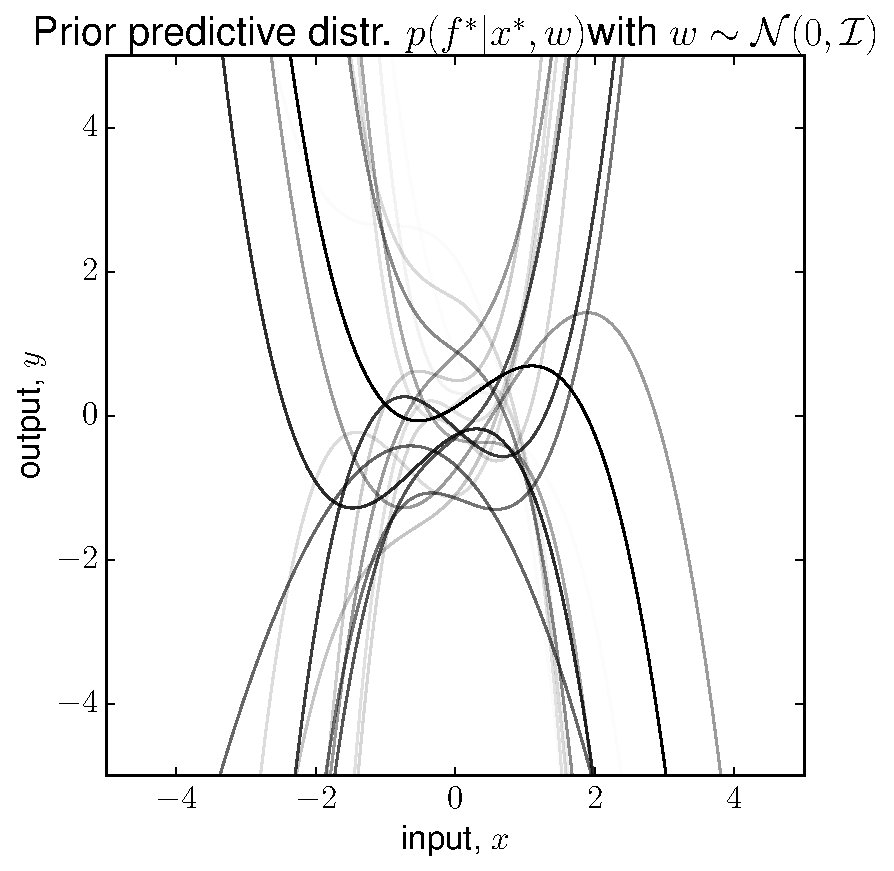
\includegraphics[width=0.5\textwidth]{images/plots/feat_space_prior.pdf} &
        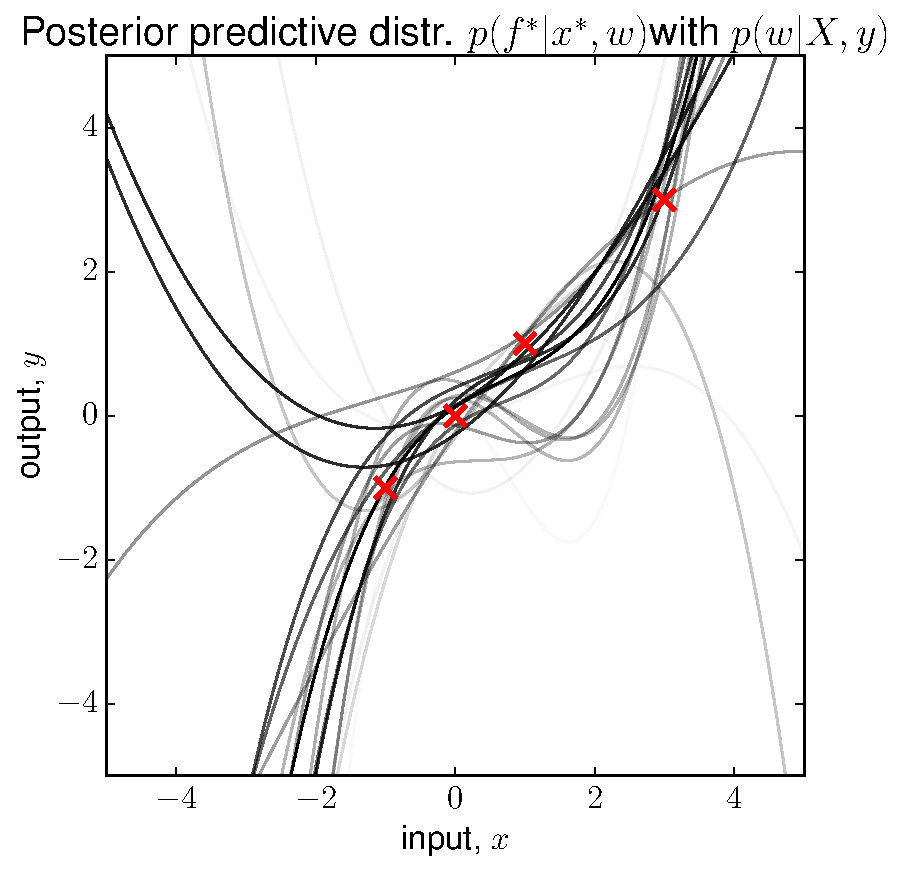
\includegraphics[width=0.5\textwidth]{images/plots/feat_space_posterior.pdf} 
    \end{tabular}
\end{figure}
\end{frame}

%%%%%%%%%%%%%%%%%%%%%%%%%%%%%%%%%%%%%%%%%%%%%%%%%%%%%%%%%%%%%%%%%%%%%%%%%

\begin{frame}
\frametitle{Rewriting this equation using a kernel (1)}
In \eqref{eq:posterior_pred_dist_basis}, we have to invert the $N \times N$ matrix $A$\\
(where $N$ = number of dimensions, or basis functions):
%
\begin{equation*}
f_{\star} | \bx_{\star}, \bX, \by \sim \norm(\frac{1}{\sigma_n^2} \phi(\bx_{\star})\transpose A\inv \Phi \by,
\phi(\bx_{\star})\transpose A\inv \phi(\bx_{\star}))
\end{equation*}
%
We can rewrite this equation to instead have to invert a $n \times n$ matrix (where $n$ = number of data
points):
%
\renewcommand\theequation{2.\thedefcounter}
\setcounter{defcounter}{12}
\begin{align}
f_{\star} | \bx_{\star}, \bX, \by \sim \norm (&\phi_{\star}\transpose \Sigma_p \Phi(\Phi\transpose \Sigma_p \Phi + \sigma_n^2I)^{-1}\by, \\
\nonumber{} & \phi_{\star}\transpose \Sigma_p\phi_{\star} - \phi_{\star}\transpose \Sigma_p \Phi(\Phi\transpose \Sigma_p \Phi + \sigma_n^2I)\inv
\Phi\transpose \Sigma_p \phi_{\star}),
\end{align}
%
with shorthand notation $\phi_{\star}$.
%= \phi(\bx_{\star})$ and we defined $K = \Phi\transpose \Sigma_p \Phi$.

\alert{You will derive this equivalence as part of this week's exercise.}

\end{frame}
%%%%%%%%%%%%%%%%%%%%%%%%%%%%%%%%%%%%%%%%%%%%%%%%%%%%%%%%%%%%%%%%%%%%%%%%%

\begin{frame}
\frametitle{Rewriting this equation using a kernel (2)}

\renewcommand\theequation{2.\thedefcounter}
\setcounter{defcounter}{12}
\begin{align}
f_{\star} | \bx_{\star}, \bX, \by \sim \norm (&\phi_{\star}\transpose \Sigma_p \Phi(\Phi\transpose \Sigma_p \Phi + \sigma_n^2I)^{-1}\by, \\
\nonumber{} & \phi_{\star}\transpose \Sigma_p\phi_{\star} - \phi_{\star}\transpose \Sigma_p \Phi(\Phi\transpose \Sigma_p \Phi + \sigma_n^2I)\inv
\Phi\transpose \Sigma_p \phi_{\star}),
\end{align}
%
with shorthand notation $\phi_{\star} = \phi(\bx_{\star})$.

%and we defined $K = \Phi\transpose \Sigma_p \Phi$.


\vspace*{0.5cm}
Note that the features $\phi(\bx_{\star})$ only enter this equation in the forms of $\phi_{\star}\transpose \Sigma_p \Phi$, $\phi_{\star}\transpose \Sigma_p\phi_{\star}$, and $\Phi\transpose \Sigma_p \Phi$. 

We can replace all of these occurrences by expressions of the form 
\vspace*{-0.2cm}
\begin{equation}
\nonumber k(\bx_1, \bx_2) = \phi(\bx_1)\transpose \Sigma_p \phi(\bx_2)   
\end{equation}
\vspace*{0.1cm}
This is known as the \alert{kernel trick}. Then, the equation becomes:

\vspace*{-0.3cm}
\begin{align}
f_{\star} | \bx_{\star}, \bX, \by \sim \norm (& k_{\star}\transpose (K + \sigma_n^2I)^{-1}\by, \\
\nonumber{} & k_{\star\star} - k_{\star}\transpose(K + \sigma_n^2I)\inv
k_{\star}.
\end{align}

\end{frame}
%%%%%%%%%%%%%%%%%%%%%%%%%%%%%%%%%%%%%%%%%%%%%%%%%%%%%%%%%%%%%%%%%%%%%%%%%





%%%%%%%%%%%%%%%%%%%%%%%%%%%%%%%%%%%%%%%%%%%%%%%%%%%%%%%%%%%%%%%%%%%%%%%%%
\section{Gaussian processes: the function space view}
\begin{frame}
\frametitle{Gaussian process}
\begin{definition}[Gaussian process]
A \alert{Gaussian process (GP)} is a collection of random variables, any finite number of which have a joint Gaussian distribution.
\end{definition}

A GP is completely specified by its mean and covariance function:
\renewcommand\theequation{2.\thedefcounter}
\setcounter{defcounter}{13}
\begin{align*}
           m(\bx) =& \mathds{E} \left[ f(\bx) \right], \\
\nonumber{} k(\bx, \bx') =& \mathds{E} \left[ (f(\bx) - m(\bx)) (f(\bx') - m(\bx')) \right]  
\end{align*}

The GP is then:
\renewcommand\theequation{2.\thedefcounter}
\setcounter{defcounter}{14}
\begin{equation}
f(\bx) \sim \mathcal{GP}(m(\bx), k(\bx, \bx'))
\end{equation}

\end{frame}

%%%%%%%%%%%%%%%%%%%%%%%%%%%%%%%%%%%%%%%%%%%%%%%%%%%%%%%%%%%%%%%%%%%%%%%%%
\begin{frame}
\frametitle{The Bayesian linear regression model is a GP}
The prior Bayesian linear model (before seeing any data $\bX, \by$) is:
%
\renewcommand\theequation{2.\thedefcounter}
\setcounter{defcounter}{15}
\begin{align}
\mathds{E} \left[ f(\bx) \right] =& \phi(\bx)^T \mathds{E} \left[ \bw \right] = 0 \\
\nonumber{} \mathds{E} \left[ f(\bx) f(\bx') \right] =& \phi(\bx)\transpose \mathds{E} \left[ \bw \bw\transpose \right] \phi(\bx') =
\phi(\bx)^T \Sigma_p \phi(\bx')
\end{align}
%
Thus $f(\bx)$ and $f(\bx')$ are jointly Gaussian with mean zero and \alert{covariance function} $k(\bx, \bx') = \phi(\bx)\transpose \Sigma_p \phi(\bx')$
\end{frame}

%%%%%%%%%%%%%%%%%%%%%%%%%%%%%%%%%%%%%%%%%%%%%%%%%%%%%%%%%%%%%%%%%%%%%%%%%
\begin{frame}
\frametitle{The squared exponential (SE) covariance}
Many different covariance functions (or \alert{kernel functions}) are possible; a prominent one is the squared
exponential (SE) covariance function:
\renewcommand\theequation{2.\thedefcounter}
\setcounter{defcounter}{16}
\begin{equation}
cov(f(\bx_p), f(\bx_q)) = k(\bx_p, \bx_q) = \exp \left(-\frac{1}{2} |\bx_p - \bx_q|^2 \right)
\end{equation}
\begin{itemize}
  \item Points that are close to each other have correlation $\approx 1$
  \item Points that are far away from each other have correlation $\approx 0$
  \item This gives rise to very smooth functions
\end{itemize}
\end{frame}

%%%%%%%%%%%%%%%%%%%%%%%%%%%%%%%%%%%%%%%%%%%%%%%%%%%%%%%%%%%%%%%%%%%%%%%%
\begin{frame}
\frametitle{Samples from the GP prior}
Samples for a finite number of points $\bX_{\star}$
\begin{equation*}
\bm{f}_{\star} \sim \norm \left(\bm{0}, K( \bX_{\star}, \bX_{\star} )\right)
\end{equation*}
Thus, we're just sampling from a multivariate Gaussian distribution. For visualization, we connect the dots.

\begin{figure}
    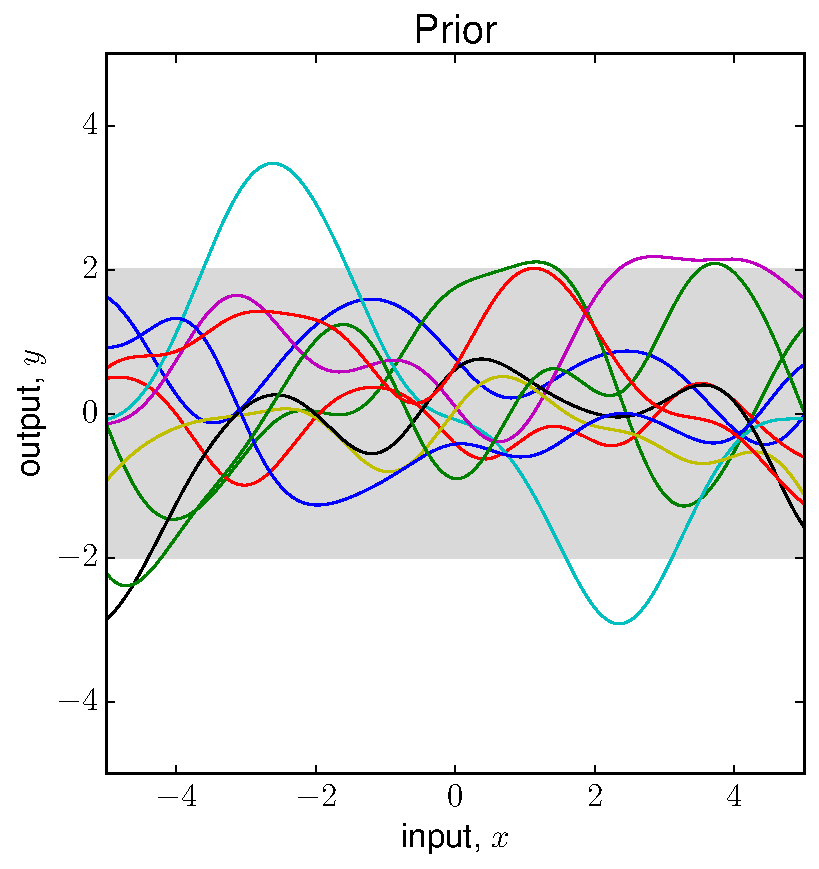
\includegraphics[width=0.4\textwidth]{images/plots/fct_space_prior_wo_noise.pdf}
\end{figure}

\end{frame}

%%%%%%%%%%%%%%%%%%%%%%%%%%%%%%%%%%%%%%%%%%%%%%%%%%%%%%%%%%%%%%%%%%%%%%%%%

\subsection{The Case of Noise-free Observations}
\begin{frame}
\tableofcontents[currentsubsection]
\end{frame}

%%%%%%%%%%%%%%%%%%%%%%%%%%%%%%%%%%%%%%%%%%%%%%%%%%%%%%%%%%%%%%%%%%%%%%%%%

\begin{frame}
\frametitle{Prediction with Noise-free Observations}
Observed function values $f$ and new function values $f_{\star}$ are jointly Gaussian-distributed
\begin{equation*}
\begin{bmatrix}
\bm{f}\\
\bm{f}_{\star}
\end{bmatrix}
\sim \norm\left(
\bm{0},
\begin{bmatrix}
K(\bX, \bX) & K(\bX, \bX_{\star})\\
K(\bX_{\star}, \bX) & K(\bX_{\star}, \bX_{\star})
\end{bmatrix}
\right)
\end{equation*}
\\
We simply apply the formula for conditioning a Gaussian to compute the predictive distribution
$\bm{f}_{\star} | \bm{f}$:
%
\renewcommand\theequation{2.\thedefcounter}
\setcounter{defcounter}{19}
\begin{align}
\bm{f}_{\star} | \bX_{\star}, \bX, \bm{f} \sim \norm(& K(\bX_{\star}, \bX) K(\bX, \bX)\inv \bm{f},\\
\nonumber{} &K(\bX_{\star}, \bX_{\star}) - K(\bX_{\star}, \bX) K(\bX, \bX)\inv K(\bX, \bX_{\star}))
\end{align}
%
\end{frame}

%%%%%%%%%%%%%%%%%%%%%%%%%%%%%%%%%%%%%%%%%%%%%%%%%%%%%%%%%%%%%%%%%%%%%%%%%


\begin{frame}
\frametitle{Samples from prior and posterior}
Intuitively, we draw many (infinitely many) samples from the prior and discard those that don't agree
perfectly with the noise-free data points
\begin{figure}
    \begin{tabular}{cc}
        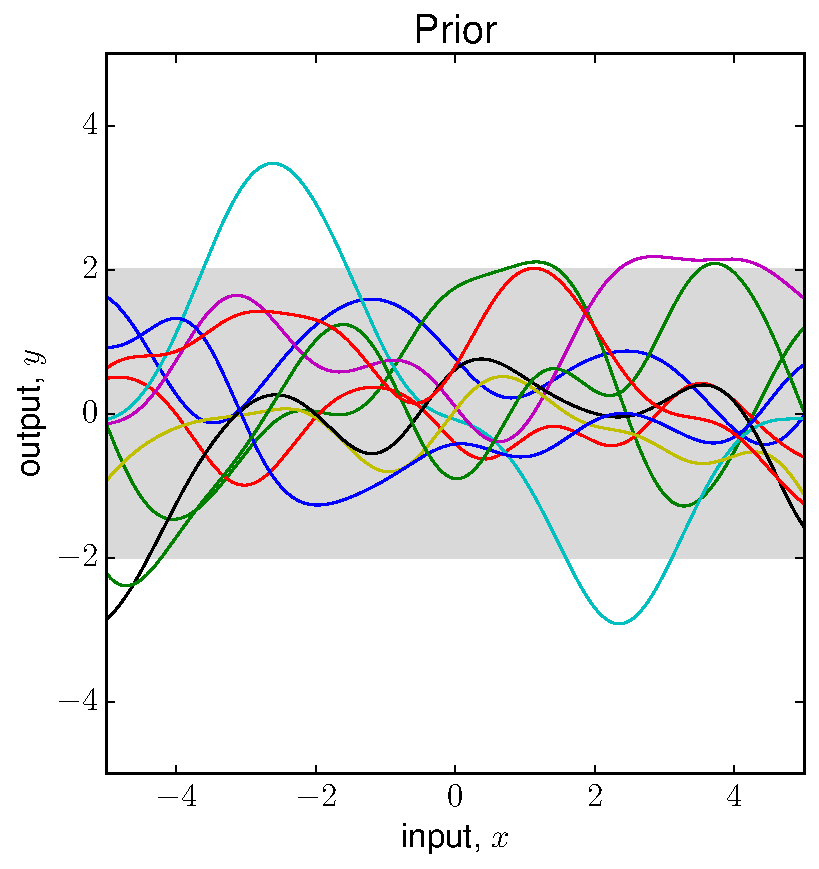
\includegraphics[width=0.45\textwidth]{images/plots/fct_space_prior_wo_noise.pdf} &
        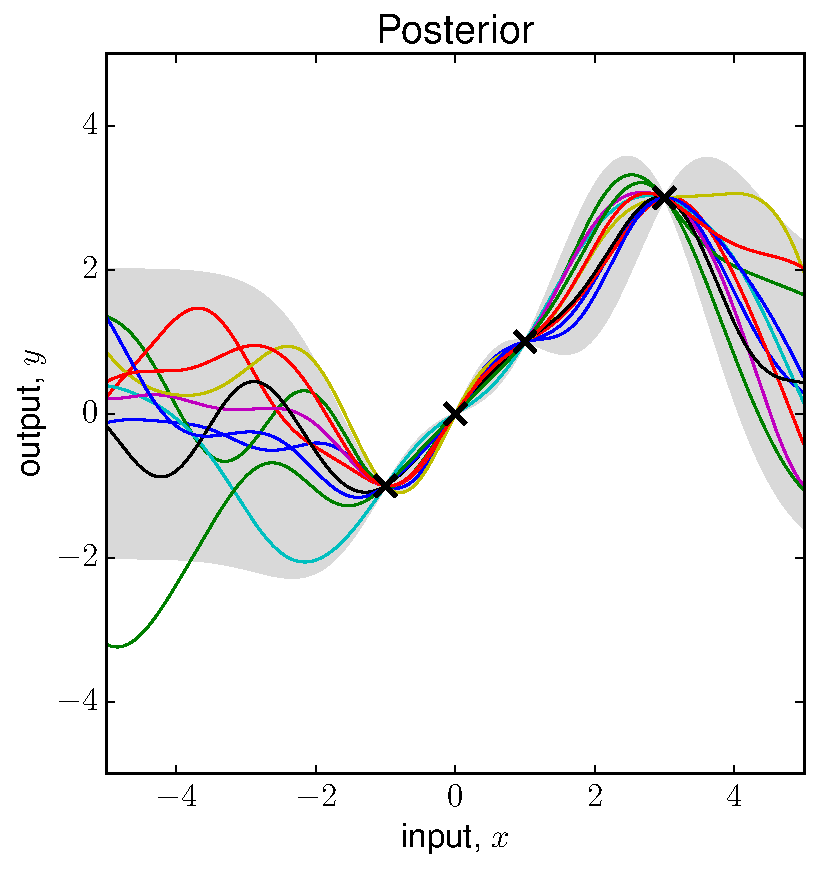
\includegraphics[width=0.45\textwidth]{images/plots/fct_space_posterior_wo_noise.pdf}
    \end{tabular}
\end{figure}
\end{frame}


%%%%%%%%%%%%%%%%%%%%%%%%%%%%%%%%%%%%%%%%%%%%%%%%%%%%%%%%%%%%%%%%%%%%%%%%%

%%%%%%%%%%%%%%%%%%%%%%%%%%%%%%%%%%%%%%%%%%%%%%%%%%%%%%%%%%%%%%%%%%%%%%%%%

\subsection{The Case of Noisy Observations}
\begin{frame}
\tableofcontents[currentsubsection]
\end{frame}

%%%%%%%%%%%%%%%%%%%%%%%%%%%%%%%%%%%%%%%%%%%%%%%%%%%%%%%%%%%%%%%%%%%%%%%%%

\begin{frame}
\frametitle{Now we have noisy observations}
As in the case of Bayesian liner regression:\\
we'll assume i.i.d Gaussian noise with variance $\sigma_n^2$
%
\begin{align*}
y =&~ f(\bx) + \epsilon \\
\epsilon \sim&~ \norm(0, \sigma_n^2)
\end{align*}
%
The prior on the noise observations is:
\renewcommand\theequation{2.\thedefcounter}
\setcounter{defcounter}{20}
\begin{align}
\nonumber{} cov(y_p, y_q) =&~ k(\bx_p, \bx_q) + \sigma_n^2 \delta_{pq} \\
cov(\by) =&~ K(\bX, \bX) + \sigma_n^2 I
\end{align}
%
Thus:
\renewcommand\theequation{2.\thedefcounter}
\setcounter{defcounter}{21}
\begin{equation}
\begin{bmatrix}
\bm{y}\\
\bm{f}_{\star}
\end{bmatrix}
\sim \norm\left(
\bm{0},
\begin{bmatrix}
K(\bX, \bX) + \sigma_n^2 I & K(\bX, \bX_{\star})\\
K(\bX_{\star}, \bX) & K(\bX_{\star}, \bX_{\star})
\end{bmatrix}
\right)
\end{equation}
\end{frame}

%%%%%%%%%%%%%%%%%%%%%%%%%%%%%%%%%%%%%%%%%%%%%%%%%%%%%%%%%%%%%%%%%%%%%%%%%

\begin{frame}
\frametitle{Predictions under noisy observations}
\renewcommand\theequation{2.\thedefcounter}
\setcounter{defcounter}{21}
\begin{equation}
\begin{bmatrix}
\bm{y}\\
\bm{f}_{\star}
\end{bmatrix}
\sim \norm\left(
\bm{0},
\begin{bmatrix}
K(\bX, \bX) + \sigma_n^2 I & K(\bX, \bX_{\star})\\
K(\bX_{\star}, \bX) & K(\bX_{\star}, \bX_{\star})
\end{bmatrix}
\right)
\end{equation}
%
Using the same equation for conditioning Gaussians as before, we derive the posterior predictive distribution:
%
\small
\renewcommand\theequation{2.\thedefcounter}
\setcounter{defcounter}{22}
\begin{equation}
f_{\star} | \bX, \by, \bX_{\star} \sim \norm(\bar{\bm{f}_{\star}}, cov(f_{\star})) \text{, where}
\end{equation}
%
\setcounter{defcounter}{23}
\begin{equation}
\bar{\bm{f}_{\star}} \triangleq \left[ f_{\star} | \bX, y, \bX_{\star} \right] = K(\bX_{\star}, \bX) \left[ K(\bX, \bX)
+ \sigma_n^2 I \right]\inv y,
\end{equation}
%
\setcounter{defcounter}{24}
\begin{equation}
cov(\bm{f}_{\star}) = K(\bX_{\star}, \bX_{\star}) - K(\bX_{\star}, \bX)\left[ K(\bX, \bX)
+ \sigma_n^2 I \right]\inv K(\bX, \bX_{\star})
\end{equation}
\normalsize
\end{frame}


%%%%%%%%%%%%%%%%%%%%%%%%%%%%%%%%%%%%%%%%%%%%%%%%%%%%%%%%%%%%%%%%%%%%%%%%%

\begin{frame}
\frametitle{The predictive distribution}
Using more compact notation, we have:
\renewcommand\theequation{2.\thedefcounter}
\setcounter{defcounter}{25}
\begin{equation}
\bar{f_{\star}} = \bk_{\star}\transpose(K + \sigma_n^2 I)\inv\by,
\end{equation}
%
\setcounter{defcounter}{26}
\begin{equation}
\mathds{V} \left[ f_{\star} \right]  = k(\bx_{\star}, \bx_{\star}) - \bk_{\star}\transpose (K + \sigma_n^2
I)\inv\bk_{\star},
\end{equation}
Note that with covariance function $\phi(\bx)\transpose \Sigma_p \phi(\bx')$ this is exactly the same as
Bayesian linear regression:
%
\setcounter{defcounter}{12}
\begin{align}
f_{\star} | \bx_{\star}, \bX, \by \sim \norm(& \phi_{\star}\transpose \Sigma_p \Phi(K + \sigma_n^2I)\inv \by,\\
\nonumber{} & \phi_{\star}\transpose \Sigma_p\phi_{\star} - \phi_{\star}\transpose \Sigma_p \Phi(K + \sigma_n^2I)\inv \Phi\transpose \Sigma_p \phi_{\star})
\end{align}
%
\end{frame}

%%%%%%%%%%%%%%%%%%%%%%%%%%%%%%%%%%%%%%%%%%%%%%%%%%%%%%%%%%%%%%%%%%%%%%%%%

\begin{frame}
\frametitle{The predictive distribution}
\renewcommand\theequation{2.\thedefcounter}
\setcounter{defcounter}{25}
\begin{equation}
\bar{f_{\star}} = \bk_{\star}\transpose(K + \sigma_n^2 I)\inv\by,
\end{equation}
\renewcommand\theequation{2.\thedefcounter}
\setcounter{defcounter}{26}
\begin{equation}
\mathds{V} \left[ f_{\star} \right]  = k(\bx_{\star}, \bx_{\star}) - \bk_{\star}\transpose (K + \sigma_n^2
I)\inv\bk_{\star},
\end{equation}

Some properties of the mean
\begin{itemize}
  \item A linear combination of response values $y$
  \item A linear combination of $n$ kernel functions, each one centered on a training data point:\\

  \renewcommand\theequation{2.\thedefcounter}
  \setcounter{defcounter}{27}
  \begin{align}
  \bar{f(\bx_{\star})} &= \sum_{i=1}^n \alpha_i k(\bx_i, \bx_{\star}) \\
  \nonumber{} \text{where } \bm{\alpha} &= (K + \sigma_n^2 I)\inv \by
  \end{align}

\end{itemize}
\end{frame}

%%%%%%%%%%%%%%%%%%%%%%%%%%%%%%%%%%%%%%%%%%%%%%%%%%%%%%%%%%%%%%%%%%%%%%%%%

\subsection{Marginal likelihood and kernel hyperparameters}
\begin{frame}
\tableofcontents[currentsubsection]
\end{frame}

%%%%%%%%%%%%%%%%%%%%%%%%%%%%%%%%%%%%%%%%%%%%%%%%%%%%%%%%%%%%%%%%%%%%%%%%%

\begin{frame}
\frametitle{The marginal likelihood}
The marginal likelihood is the integral of the likelihood times the prior:
%
\renewcommand\theequation{2.\thedefcounter}
\setcounter{defcounter}{28}
\begin{equation}
p(\by | \bX) = \int{p(\by | \bm{f}, \bX) p(\bm{f}| \bX) d\bm{f}}.
\end{equation}
%
It marginalizes (integrates out) the actual function values. \\
We know that this is distributed according to a Gaussian:
\begin{equation*}
\by \sim \norm(0, K + \sigma_n^2 I)
\end{equation*}
%
Usually, one works with the log marginal likelihood:
%
\scriptsize
\renewcommand\theequation{2.\thedefcounter}
\setcounter{defcounter}{30}
\begin{equation}
\log p(\by | \bX) = - \frac{1}{2} \by\transpose (K + \sigma_n^2 I) \inv \by - \frac{1}{2} \log |K +
\sigma_n^2 I | - \frac{n}{2} \log 2 \pi
\end{equation}
\normalsize
\end{frame}

%%%%%%%%%%%%%%%%%%%%%%%%%%%%%%%%%%%%%%%%%%%%%%%%%%%%%%%%%%%%%%%%%%%%%%%%%
\begin{frame}
\frametitle{The effect of the kernel hyperparameters}
The SE covariance function in 1-d:
  \renewcommand\theequation{2.\thedefcounter}
  \setcounter{defcounter}{31}
  \begin{equation}
	k_y(x_p, x_q) = \sigma_f^2 \exp (- \frac{1}{2l^2} (x_p- x_q)^2) + \sigma_n^2 \delta_{pq}
  \end{equation}
The marginal likelihood is highest for the left plot. It trades off data fit and ``complexity'' of the function
\begin{figure}
\begin{tabular}{ccc}
    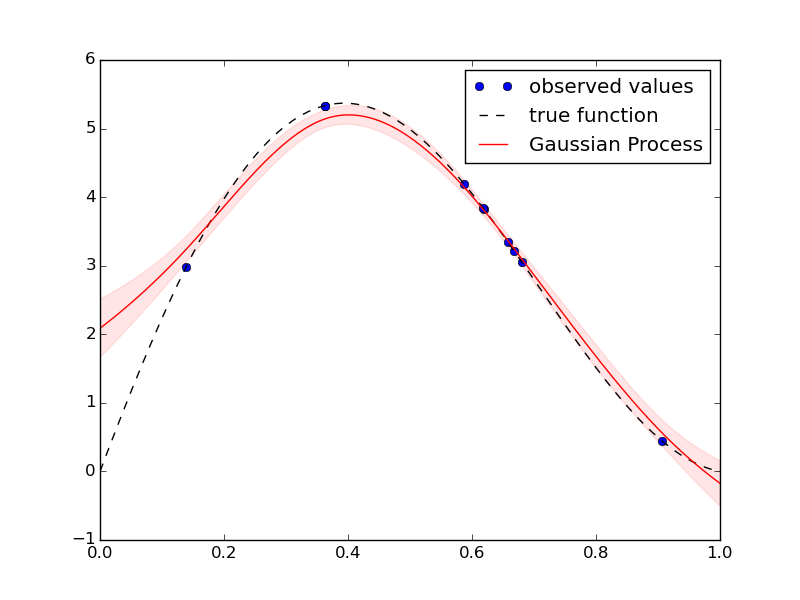
\includegraphics[width=0.3\textwidth]{images/plots/gp_kernel_params_0.png} &
    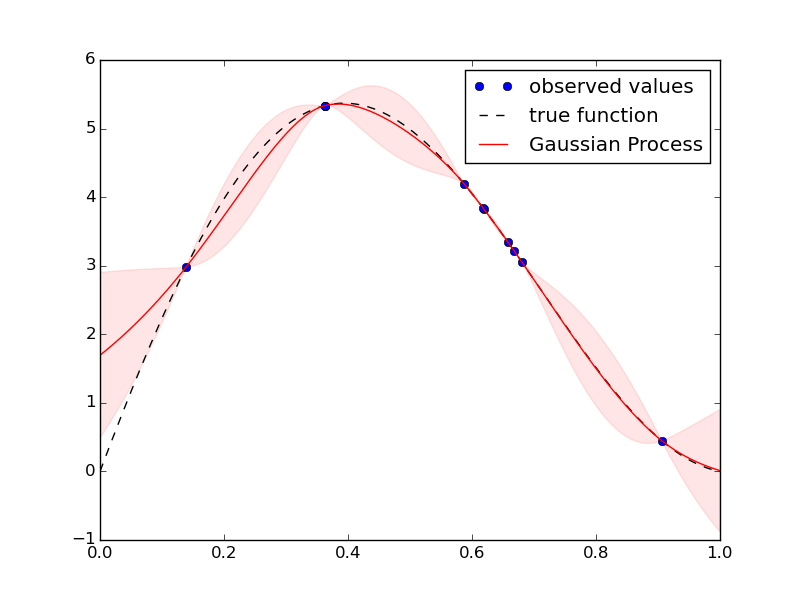
\includegraphics[width=0.3\textwidth]{images/plots/gp_kernel_params_1.png} &
    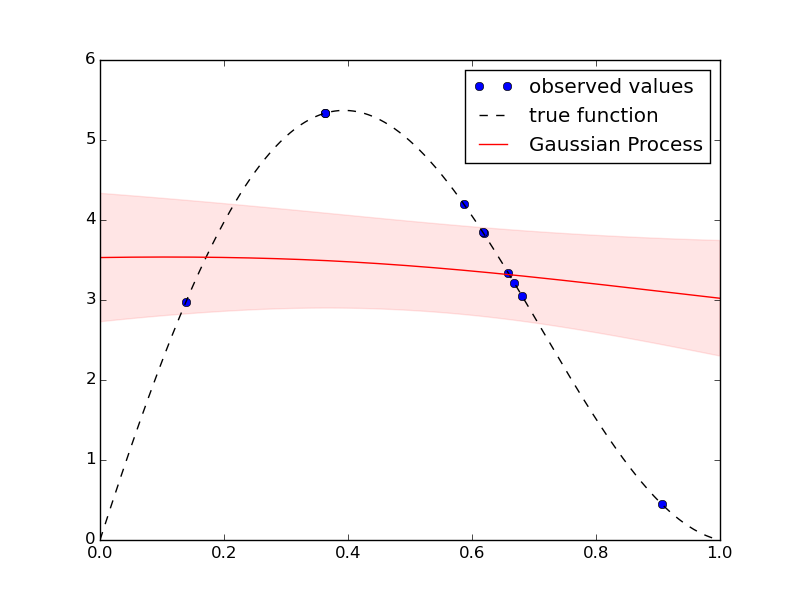
\includegraphics[width=0.3\textwidth]{images/plots/gp_kernel_params_2.png} \\
\end{tabular}
\end{figure}
\end{frame}
%%%%%%%%%%%%%%%%%%%%%%%%%%%%%%%%%%%%%%%%%%%%%%%%%%%%%%%%%%%%%%%%%%%%%%%%%

%%%%%%%%%%%%%%%%%%%%%%%%%%%%%%%%%%%%%%%%%%%%%%%%%%%%%%%%%%%%%%%%%%%%%%%%%

\begin{frame}
\frametitle{Summary by Learning Goals}
Now (after digesting the material and doing the exercise), you can \ldots
\begin{itemize}
\item Derive Bayesian linear regression
\item Derive Gaussian processes
\item Explain the relationship between Bayesian linear regression and Gaussian processes
\end{itemize}

\end{frame}

%%%%%%%%%%%%%%%%%%%%%%%%%%%%%%%%%%%%%%%%%%%%%%%%%%%%%%%%%%%%%%%%%%%%%%%%%


